\section{Experiments}
\label{sec:experiments}


In this section, we report a series of experiments in which
we explore the kinds of linguistic regularities the networks learn from
word-level input. 
%Sections~\ref{sec:computeomission} to \ref{sec:beyondlexical} 
%present the analyses of the final hidden activation 
%vectors of the recurrent pathways from a linguistic point of view. 
%Sections~\ref{sec:syntacticdim} and \ref{seq:describe} report exploratory experiments on
%the linguistic features encoded by individual hidden dimensions. 
In Section~\ref{sec:computeomission} we introduce \emph{omission scores},
a metric to measure the contribution of each token to the prediction
of the networks and in Section~\ref{sec:omitimaginet} we analyze how
these scores are distributed over dependency relations and
part-of-speech categories. 
In Section~\ref{sec:beyondlexical} we investigate the extent to which
the importance of words for the different networks depend on the words themselves,
their sequential position and their grammatical function in the sentences.
Finally, in Section~\ref{sec:contexts} we systematically compare the types of 
n-gram contexts that trigger individual dimensions in the hidden layers of the 
networks, and discuss their level of abstractness.

In all these experiments we report our findings based on the {\sc Imaginet}
model, whenever appropriate compare to our two other models {\sc LM} and {\sc Sum}, 
and discuss the generalizabilty of our methods to other architectures.
\label{edit:experimentsgeneral}
For all the experiments, we trained the models on the training portion of the
MSCOCO image-caption dataset \cite{lin2014microsoft}, and analyzed the
representations of the sentences in the validation set corresponding
to 5000 randomly chosen images. The target image representations were
extracted from the pre-softmax layer of the 16-layer CNN of
\namecite{simonyan2014very}.

% \iffalse

% {\bf Section~\ref{sec:macro}} includes experiments that provide linguistic analysis of the activation patterns on the activation vector level with results more quantitative in nature. Section~\ref{sec:salience} describes a method to estimate the salience of tokens as a function of their part-of-speech category and grammatical function (dependency relation) in sentences. 

%  Sections~\ref{sec:gramfunc} and \ref{subsec:information-struct} apply this method and provide evidence that the {\sc Visual} pathway of {\sc Imaginet} learns to interpret the same word fullfilling different grammatical functions differently, and is sensitive to the information structure of sentences.


% {\bf Section~\ref{sec:micro}} compliments the macro level analysis and reports a series of more qualitative experiments exploring the kinds of linguistic abstraction represented by individual hidden units. Section~\ref{sec:reprdim} proposes a simple method for representing
% the function of hidden units by identifying the top K contexts that yield the highest activation values, and Section~\ref{sec:topk} provides a general qualitative analysis of these contexts.

% For the experiments using the {\sc Imaginet} model we use the validation set of MS-COCO.
% Finally Section~\ref{sec:syntacticdim} goes more into detail and shows examples 
% of hidden units that are active for particular multi-word constructions with joint
% semantical and syntactic regularities.  
% \fi





%\begin{enumerate}
%\item How accurately does each model represent syntactic knowledge? WE DONT DO THIS
%\item What types of grammatical functions each model pays most attention to? WE DO THIS
%\item What is the level of separation between syntactic and semantic 
%representations learned by the models? NO CHANCE
%\item What functions are the individual units in each network specialized for? WE DO THIS 
%\item On each of the above dimensions, what are the systematic differences 
%between models that are optimized for different tasks?  WE ALSO DO THIS
%\end{enumerate}



%Section~\ref{sec:categories} looks at the salience of two sets of syntactic categories in 
%each model, by estimating how much input tokens from each category influence 
%the final performance in each task. In Section~\ref{sec:syntax}, we examine the 
%degree to which syntactic information is encoded in the internal representations 
%acquired by each model. Section~\ref{sec:dimension} focuses on analyzing the 
%reaction patterns of individual units in each model, and on finding out specialized 
%functions that these units perform. 

%Finally in Section~\ref{sec:visualize}, we look at 
%how the meaning representations of word sequences evolve over time for each 
%model. \todo{not sure how to relate this last one to our objectives.}
%In all our experiments, we compare the nature and degree of the acquired 
%syntactic knowledge among models that are trained for performing different tasks.


%\noindent{\bf Syntactic categories.} In all the following analyses, we use two different sets of syntactic categories: part-of-speech categories (POS) and dependency relations (DepRel). The tagging is performed jointly using the TurboParser dependency parser\footnote{This implementation is available at https://github.com/andre-martins/TurboParser.} \cite{martins2013turning}. For POS tags we use the Penn Treebank tagset and for the dependency relations the Stanford basic dependencies.



%\section{Representing syntactic information}
\label{sec:regression}

It is assumed that to perform a task that involves some level of language 
understanding, RNNs need to learn some level syntactic knowledge from the 
linguistic input. To uncover if the networks indeed represent syntactic 
information, we trained a number of Logistic Regression models on various 
combinations of n-gram tokens in the input as well as the hidden states of the 
networks to predict the syntactic categories of the tokens at each time-step $t$. 
From the sentences we extracted unigram and n-gram features up to a window 
size of 4; for example, to predict the label for {\it dog} in the sentence {\it the nice 
dog} we extract {\it the}$_2$, {\it nice}$_1$, {\it dog}$_0$, {\it the$_2$ nice$_1$}, 
{\it nice$_1$ dog$_0$}, and {\it the$_2$ nice$_1$ dog$_0$}, etc. 

We trained several models on a combination of the following features:
\begin{itemize}
  \item current word $w_t$
  \item current word-embedding of {\sc Imaginet} $e_t^I$ (same for {\sc Visual} 
and {\sc Textual})
  \item current word-embedding of {\sc Sentiment} $e_t^S$
  \item 4-gram features
  \item hidden state of {\sc Visual} $h_t^V$
  \item hidden state of {\sc Textual} $h_t^T$
  \item hidden state of {\sc Sentiment} $h_t^S$
%  \item hidden state of {\sc Visual} $h_t^V$ + 4-gram features
%  \item hidden state of {\sc Textual} $h_t^T$ + 4-gram features
\end{itemize}

The motivation behind this experiment is that if the networks generalize over 
syntactic categories, then using their activation vectors as features will lead to a 
more accurate model f$h_t$or syntactic category prediction than only using the tokens 
themselves. If the embeddings $e_t$ and hidden activations $h_t$ outperform 
the word form $w_t$ and 4-gram models respectively, then the linguistic 
representations of the model do generalize over syntactic categories.


\begin{table}[]
\centering
\caption{Results of predicting syntactic categories for each token in the input to 
SENTIMENT and IMAGINET models, by Logistic Regression classifiers trained 
on features in the first column. The second and third columns report the micro F-
scores on DepRel and POS categories respectively.}

\label{tab:logistic}
\begin{tabular}{lll}
\hline
 \multicolumn{3}{c}{\sc Sentiment}           \\
 \hline 
{\bf Features}      &  {\bf deprel} &  {\bf POS}     \\
\hline 
word $w_t$                   		  & .50  & .65   \\
4-gram                       		  & .62  & .71   \\
$e^S_{t}$          & .33  & .38   \\ 
$h_t^S$                      		  & .30  & .32    \\
\hline 
\hline
\multicolumn{3}{c}{\sc Imaginet}                          \\
 \hline 
{\bf Features}      &  {\bf deprel} &  {\bf POS}     \\
\hline 
$w_t$                   		  	      & .710   & .93  \\
4-gram                         		  & .807  & .93  \\
$e^I_{t}$          			  	      & .73   & .95  \\ 
$h_t^V$                      		  & .751  & .88  \\
$h_t^T$                      		  & .811  & .94  \\
$h_t^T$ + $h_t^V$            		  & .81   & .94  \\
$h_t^V$ + 4-gram             		  & .809   & .93  \\
$h_t^T$ + 4-gram             		  & .823   & .95
\end{tabular}
\end{table}

Table~\ref{tab:logistic} shows the results of predicting the syntactic categories of 
tokens in the input sentences using different (combinations of) features. 
\todo{Are we going to change this to test set?}

The results for {\sc Sentiment} show that the representations (both 
$e^S_{t}$ and $h_t^S$) are less predictive of the grammatical categories of the 
target words than using the unigram and 4-gram features.

%In fact there are only 8 categories out of 44 with non-zero f-scores for deprels: 
%amod (0.28), cc (.64), conj (.13), det (.56), nsubj (.29), pobj (.30), prep (.43) and 
%root (.26).
However, in case of {\sc Imaginet}, using the embeddings $e_t$ leads to higher F-score for both dependency category and part-of-speech tag prediction of the tokens $w_t$ than using $w_{t}$'s 
themselves. This result provides evidence that syntactic information is indeed encoded in the learned word embeddings. 
Similarly, the classifier trained on the hidden activations of {\sc Textual } $h_t^T$ 
performs better on both DepRel and POS prediction than using 4-grams features, but only by a 
narrow margin. 

The more interesting results, however, are the low F-scores when 
using $h_{t}^V$ as features. These results suggest that {\sc Visual} represents less 
syntactic information then {\sc Textual} about sequences of words. We also observe 
that the maximum F-score is achieved using the combinations of $h_{t}^T$ and the 4-
gram features, suggesting that perhaps some information about the word identities is 
lost in $h_{t}^T$.

%\section{Analysis of hidden activation vectors}
%\label{sec:macro}

% \begin{figure*}[t]
% \hspace*{-0.5in}
% \setlength{\tabcolsep}{0.01pt}
%     \begin{tabular}{cccc}
%     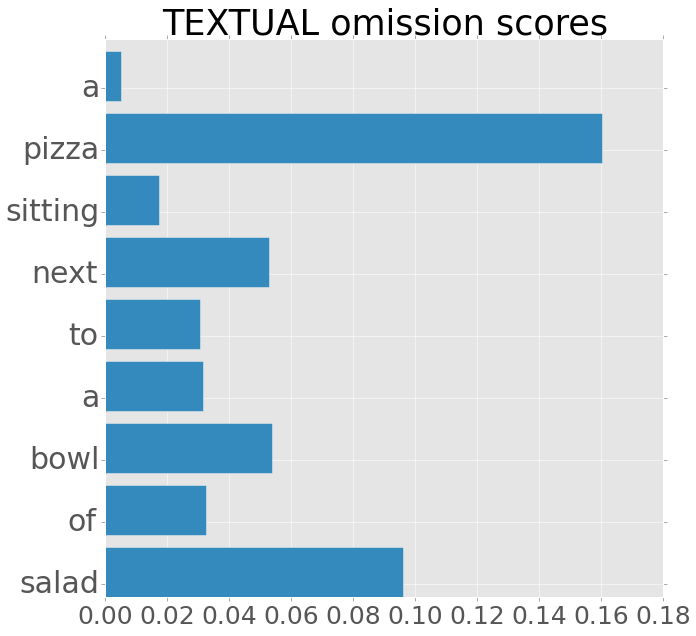
\includegraphics[scale=0.14]{new_omission_examples/textual1} &
%     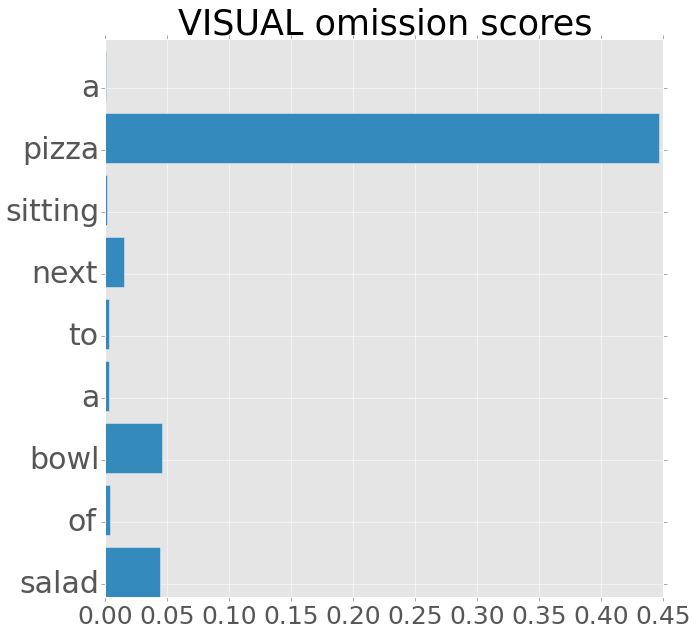
\includegraphics[scale=0.14]{new_omission_examples/visual1} &
%     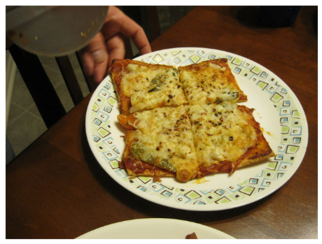
\includegraphics[scale=0.33]{new_omission_examples/img1} & 
%     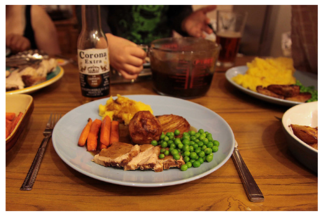
\includegraphics[scale=0.28]{new_omission_examples/img1_omit} \\
%     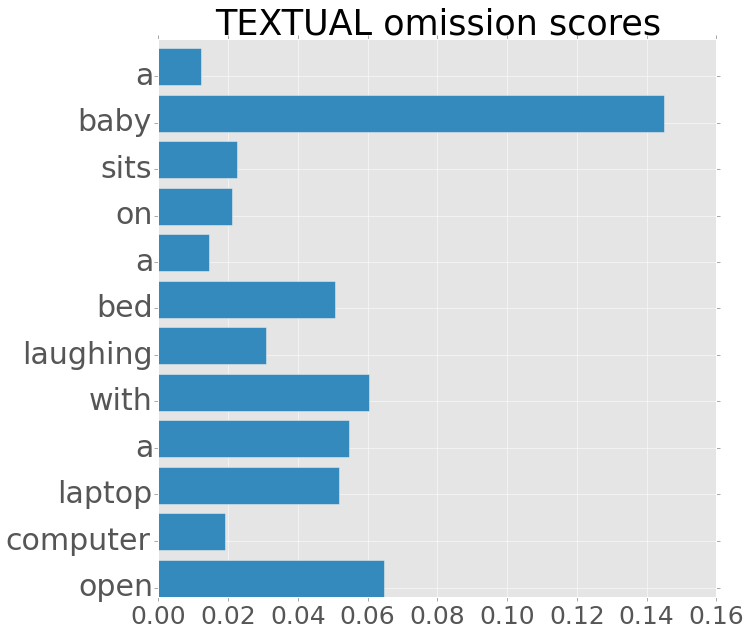
\includegraphics[scale=0.16]{new_omission_examples/textual2} &
%     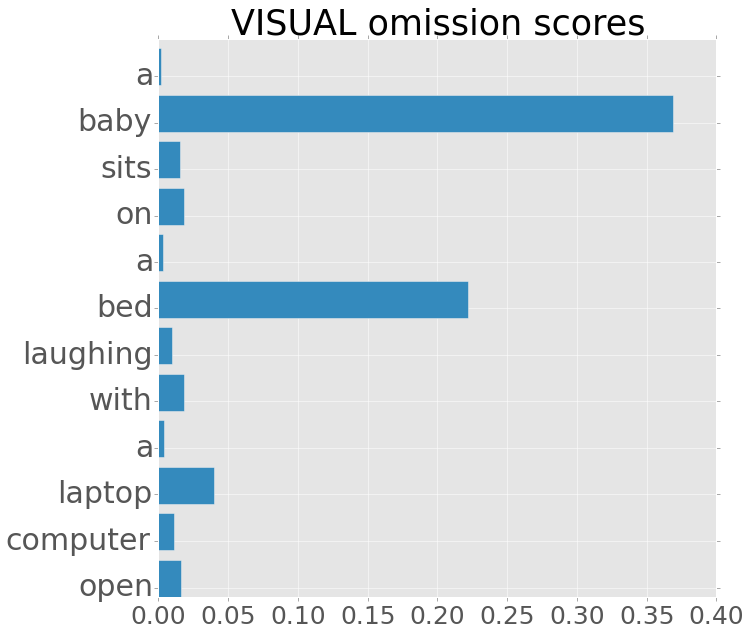
\includegraphics[scale=0.16]{new_omission_examples/visual2} &
%     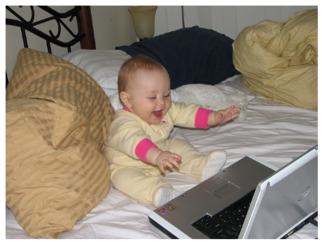
\includegraphics[scale=0.28]{new_omission_examples/img2} & 
%     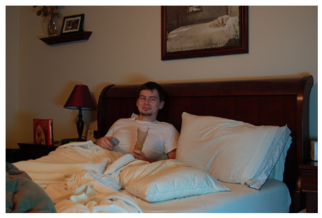
\includegraphics[scale=0.30]{new_omission_examples/img2_omit}
%     \end{tabular}
%     \caption{The omission scores of {\sc Visual} and {\sc Textual} for two example sentences, 
% and the best retrieved images for the original sentence (left) and the sentence with the most 
% important word removed (right). 
% %Top row example caption is {\it a bottle next to a windowsill with
% %  light coming through},  bottom row: {\it a train on a track next to
% %  many bushes}.
% }
%     \label{fig:omissionex}
% \end{figure*}


\begin{figure*}[t]
  \centering
  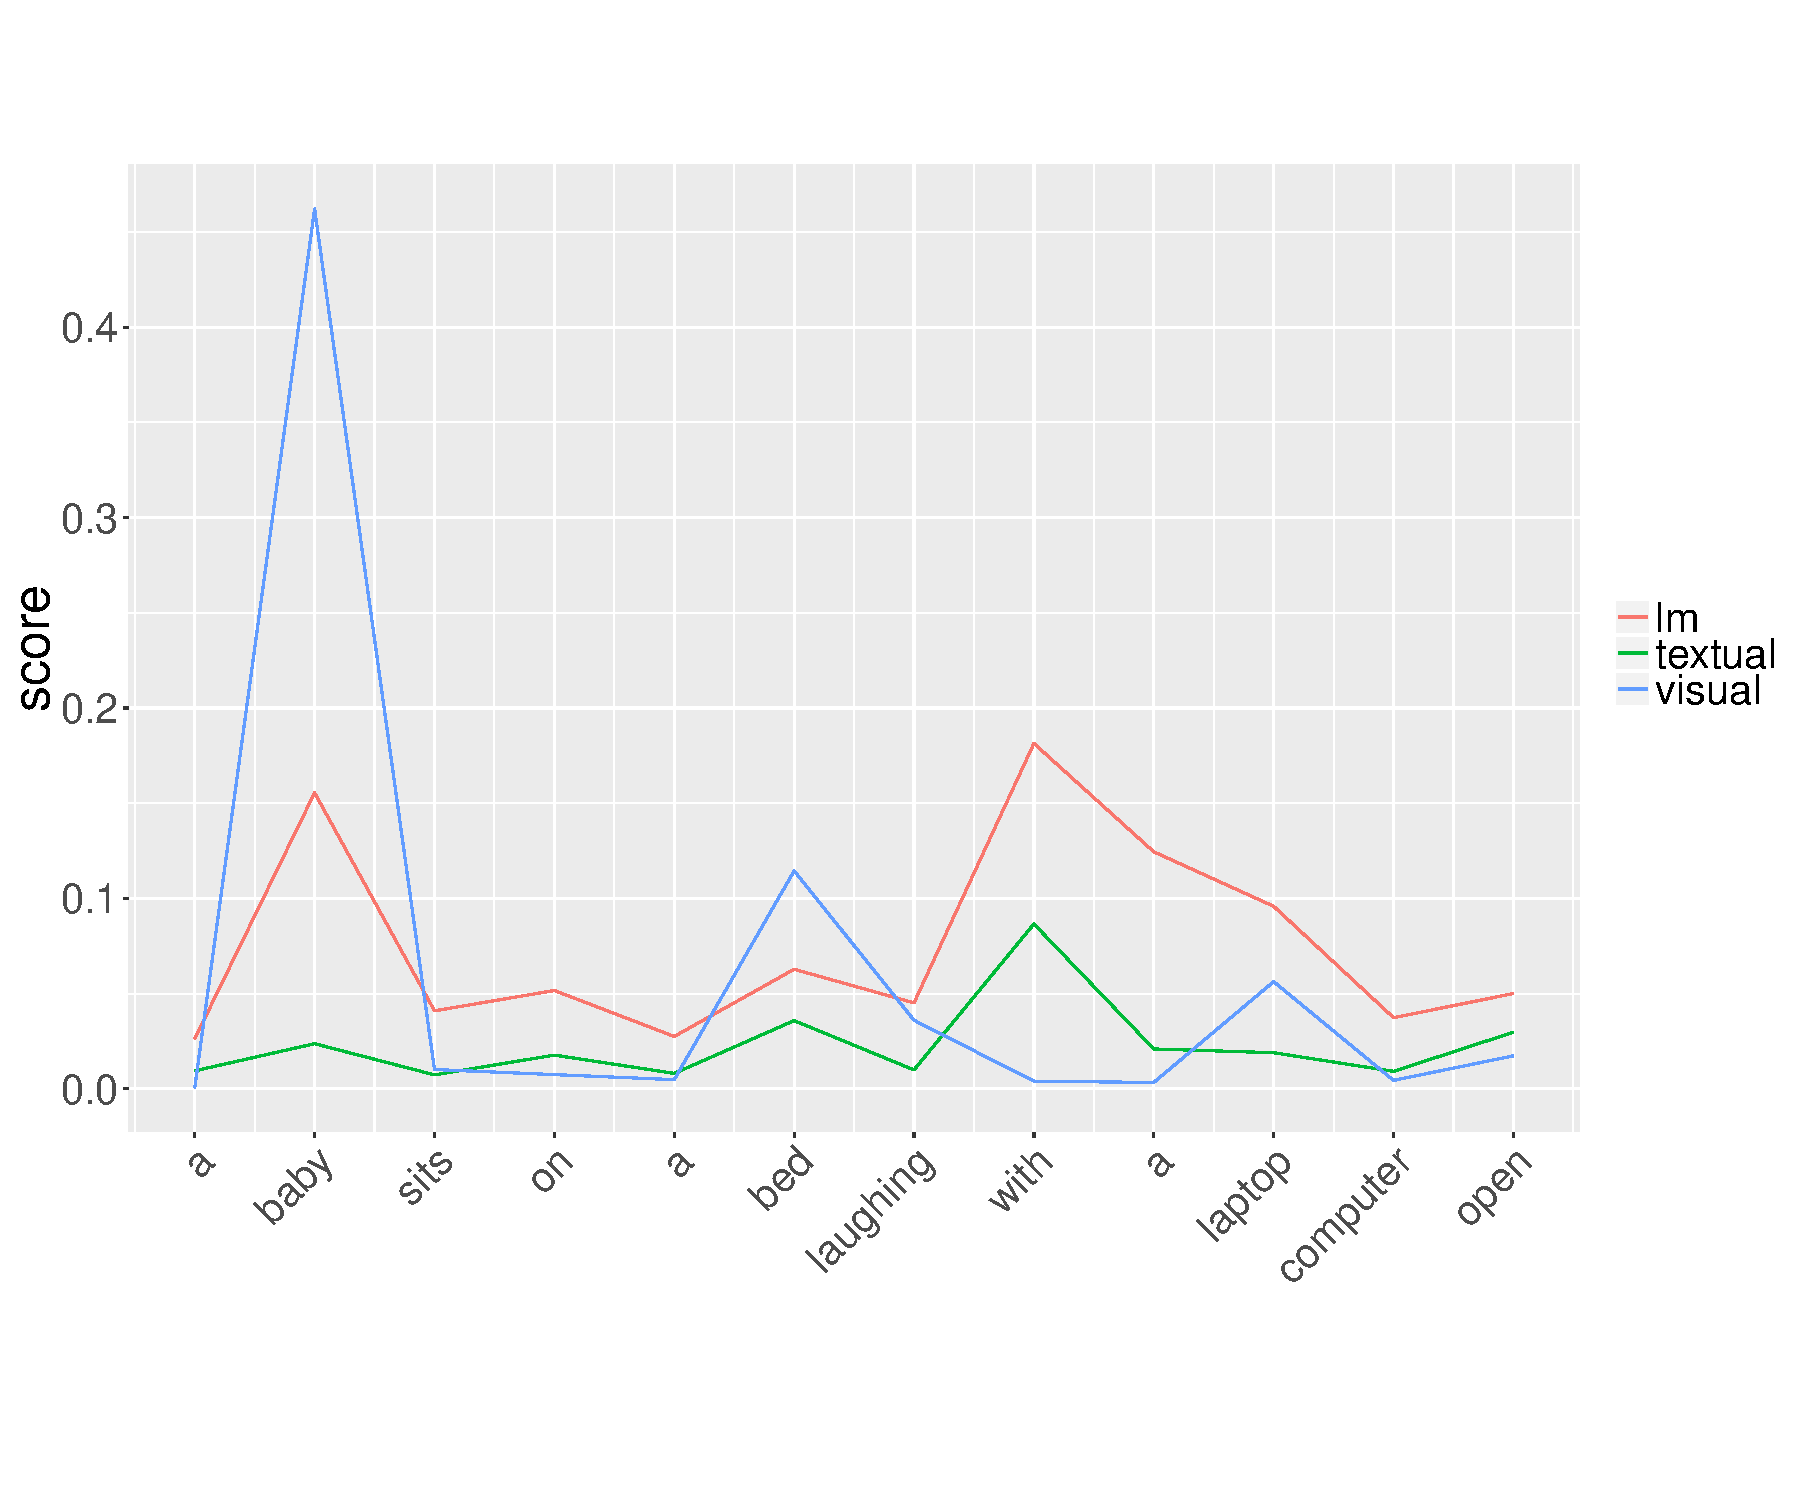
\includegraphics[scale=0.3]{omissionex.pdf}
  \caption{Omission scores for the example sentence {\it a baby sits
      on a bed laughing with a laptop computer open} for {\sc LM} and
    the two pathways, {\sc Textual} and {\sc Visual}, of {\sc
      Imaginet.}}
  \label{fig:omissionex}
\end{figure*}

\begin{figure*}[t]
  \centering
  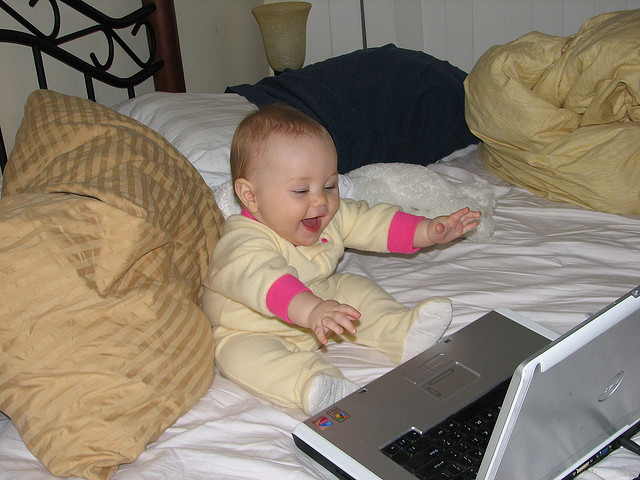
\includegraphics[scale=0.25]{85826.jpg}
  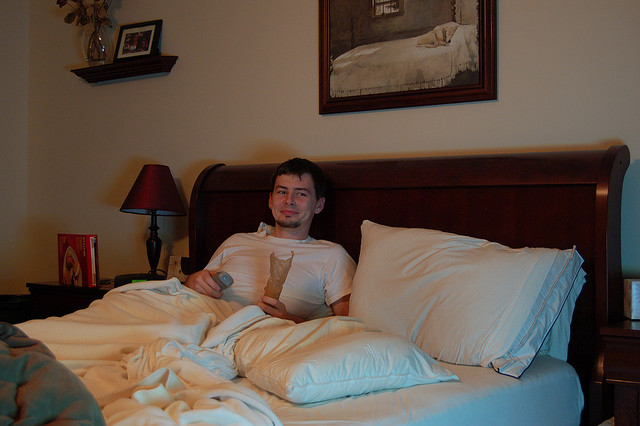
\includegraphics[scale=0.25]{60596.jpg}
  \caption{Images retrieved for the example sentence {\it a baby sits
      on a bed laughing with a laptop computer open} (left) and the
    same sentence with the second word omitted (right).}
  \label{fig:omissionexpic}
\end{figure*}





%Understanding the behavior of the learned models in terms of which features do they assign 
%the most attention to is straight forward with linear 
%models such as linear/logistic regression, 
%naive-bayes classifiers or with some of the non-parametric models as well such as decision 
%trees. This information allows researchers to not only train learning algorithms to perform 
%particular tasks, but also to uncover some underlying patterns in the training data. 
 
%\subsection{Salience of categories of words}
%\label{sec:salience}
%In this section we propose novel techniques for interpreting the
%activation patterns of neural networks trained on language tasks
%from a linguistic point of view and focus
%on the high level understanding of what parts of input sentence the networks
%pay most attention to. Furthermore, we investigate if the networks
%learn to assign differential amounts of importance to tokens depending
%on their position and grammatical function in the sentences.\label{edit:whyposdep}
%In Section~\ref{sec:computeomission} we introduce \emph{omission scores};
%a metric to measure the contribution of each token to the prediction
%of the networks and in Section~\ref{sec:omitimaginet} we analyze how
%these scores are distributed over dependency relations and
%part-of-speech categories. 
%In Section~\ref{sec:beyondlexical} we investigate the extent to which
%the importance of words for the different networks depend on the words themselves,
%their sequential position and their grammatical function in the sentences.
% MAYBE THIS WOULD BE TOO MUCH
%We apply the proposed methods to explore
%the representations of {\sc Imaginet}, but also discuss how to generalize
%them to other architectures.

\subsection{Computing Omission Scores}
\label{sec:computeomission}

We propose a novel technique for interpreting the
activation patterns of neural networks trained on language tasks
from a linguistic point of view, and focus
on the high-level understanding of what parts of input sentence the networks
pay most attention to. Furthermore, we investigate if the networks
learn to assign different amounts of importance to tokens depending
on their position and grammatical function in the sentences.\label{edit:whyposdep}

In all the models the full sentences are represented by the
activation vector at the end-of-sentence symbol
($\mathbf{h}_\text{end}$). We measure the salience of each word $S_i$
in an input sentence $S_{1:n}$ based on how much the representation of the
partial sentence $S_{\setminus i} = S_{1:i-1}S_{i+1:n}$, with
the omitted word $S_i$, deviates from that of the original sentence
representation. For example, the distance
between $\mathbf{h}_\text{end}(${\it the black dog is running}$)$
and $\mathbf{h}_\text{end}(${\it the dog is running}$)$ determines
the importance of {\it black} in the first sentence. We introduce the
measure $\mathrm{omission}(i,S)$ for estimating the salience of a word $S_i$:

\begin{equation}
\label{eg:omit}
\mathrm{omission}(i,S) = 1-\mathrm{cosine}(\mathbf{h}_\text{end}(S),
\mathbf{h}_\text{end}(S_{\setminus i}))
\end{equation}

\noindent Figure~\ref{fig:omissionex} demonstrates the omission
scores for the {\sc LM}, {\sc Visual} and {\sc Textual} models for an
example caption. The omission scores are
plotted for the
full sentence and for the sentence with the word with the highest
$\mathrm{omission}(i,S)$ removed. 
Figure~\ref{fig:omissionexpic} shows the images retrieved by {\sc
  Visual} for the full
caption and for the one with the word {\it baby} omitted. 
The images are retrieved from the validation set of MS-COCO by: 1)
computing the image representation of the given sentence with {\sc
  Visual}; 2) extracting the CNN features for the images from the set;
and 3) finding the image that minimizes the cosine distance to the
query.\label{edit:retrievalexplain} 
The omission scores for {\sc Visual} show that the model paid attention
mostly to {\it baby} and {\it bed} and slightly to {\it laptop} and
retrieved an image depicting a baby sitting on a bed with a laptop.
Removing the word {\it baby} leads to an image that depicts an adult
male laying on a bed. Figure~\ref{fig:omissionex} also shows that in
contrast to {\sc Visual}, {\sc Textual} distributes
its attention more evenly across time steps instead of focusing on the
types of words related to the corresponding visual scene. The peaks
for {\sc LM} are the same as for {\sc Textual}, but the variance of
the omission scores is higher, suggesting that the unimodal language
model is more sensitive overall to input perturbations than {\sc Textual}.


%For other RNN architectures such as LSTMs \label{edit:omitgeneral}
%and their bi-directional variants, measuring the contribution
%of tokens to their predictions (or the omission scores)
%can be straight-forwardly computed using their hidden state 
%at the last time step used for prediction. Furthermore, the technique 
%can be applied in general to other architectures which
%map variable length linguistic expressions to the same fixed dimensional
%space and perform predictions based on these embeddings. 
%This includes tree-structured Recursive Neural Network models such as the Tree-LSTM
%introduced in \namecite{kai2015treelstm} or the CNN architecture of \namecite{yoonneural2014} 
%for sentence classification. In both cases the pre-softmax activations can be extracted 
%from the models as the representations of the full and partial sentences.   


% Given a corpus segmented into sentences, each word in an input sentence is tagged with its 
%part-of-speech category (POS) and dependency-relation (DepRel). For dependency relations 
%only the label of the ark (and not the ark itself) is taken into account. For each input sentence 
%of 
%length $n$ the RNNs produce $n$ hidden activation vectors $h_{1}, \ldots , h_{n}$. Each word 
%in the input sentence is tagged with POS and DepRel categories and the contribution of the $<
%$word, POS, DepRel$>$ tuples to the meaning of the sentence is measured by computing the 
%following scores:
% 

%\paragraph{$omission$} Given a sentence "the black dog", we generate 3 sentence by 
%omitting one of the words each time: "the black", "the dog", "black dog". For each of these 
%sentence we compute a sentence representation $h_{full}$ and calculate the cosine 
%similarities 
%between the original and the omitted sentences. This measured is used to indicate the overall 
%importance of word categories. \todo{Example with a short sentence: ab, bc, cd, cosines}
%\\

%-----------------
\subsection{Omission score distributions}
\label{sec:omitimaginet}

%\begin{figure*}
 %   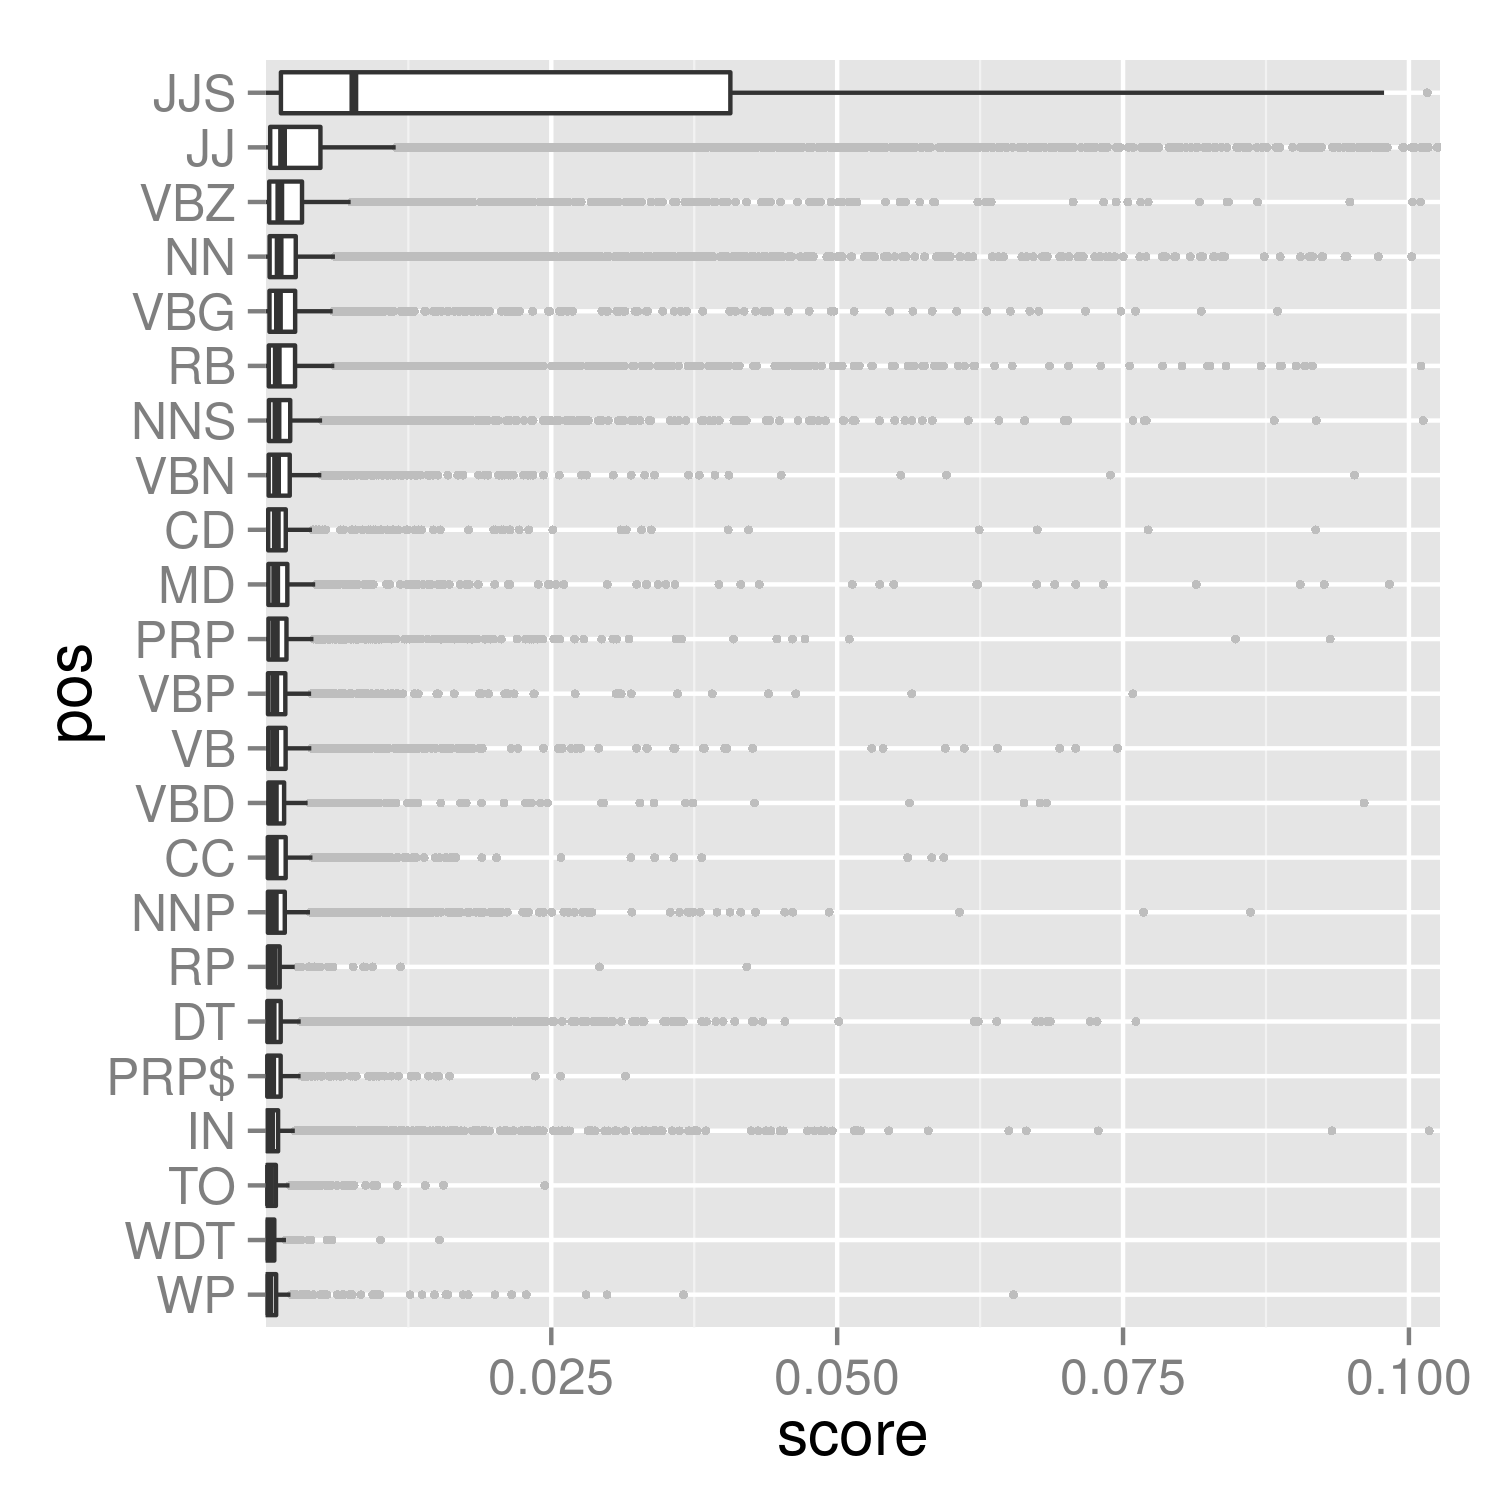
\includegraphics[scale=0.6]{omission-stat/sent-omission-pos-boxplot.png} 
 %   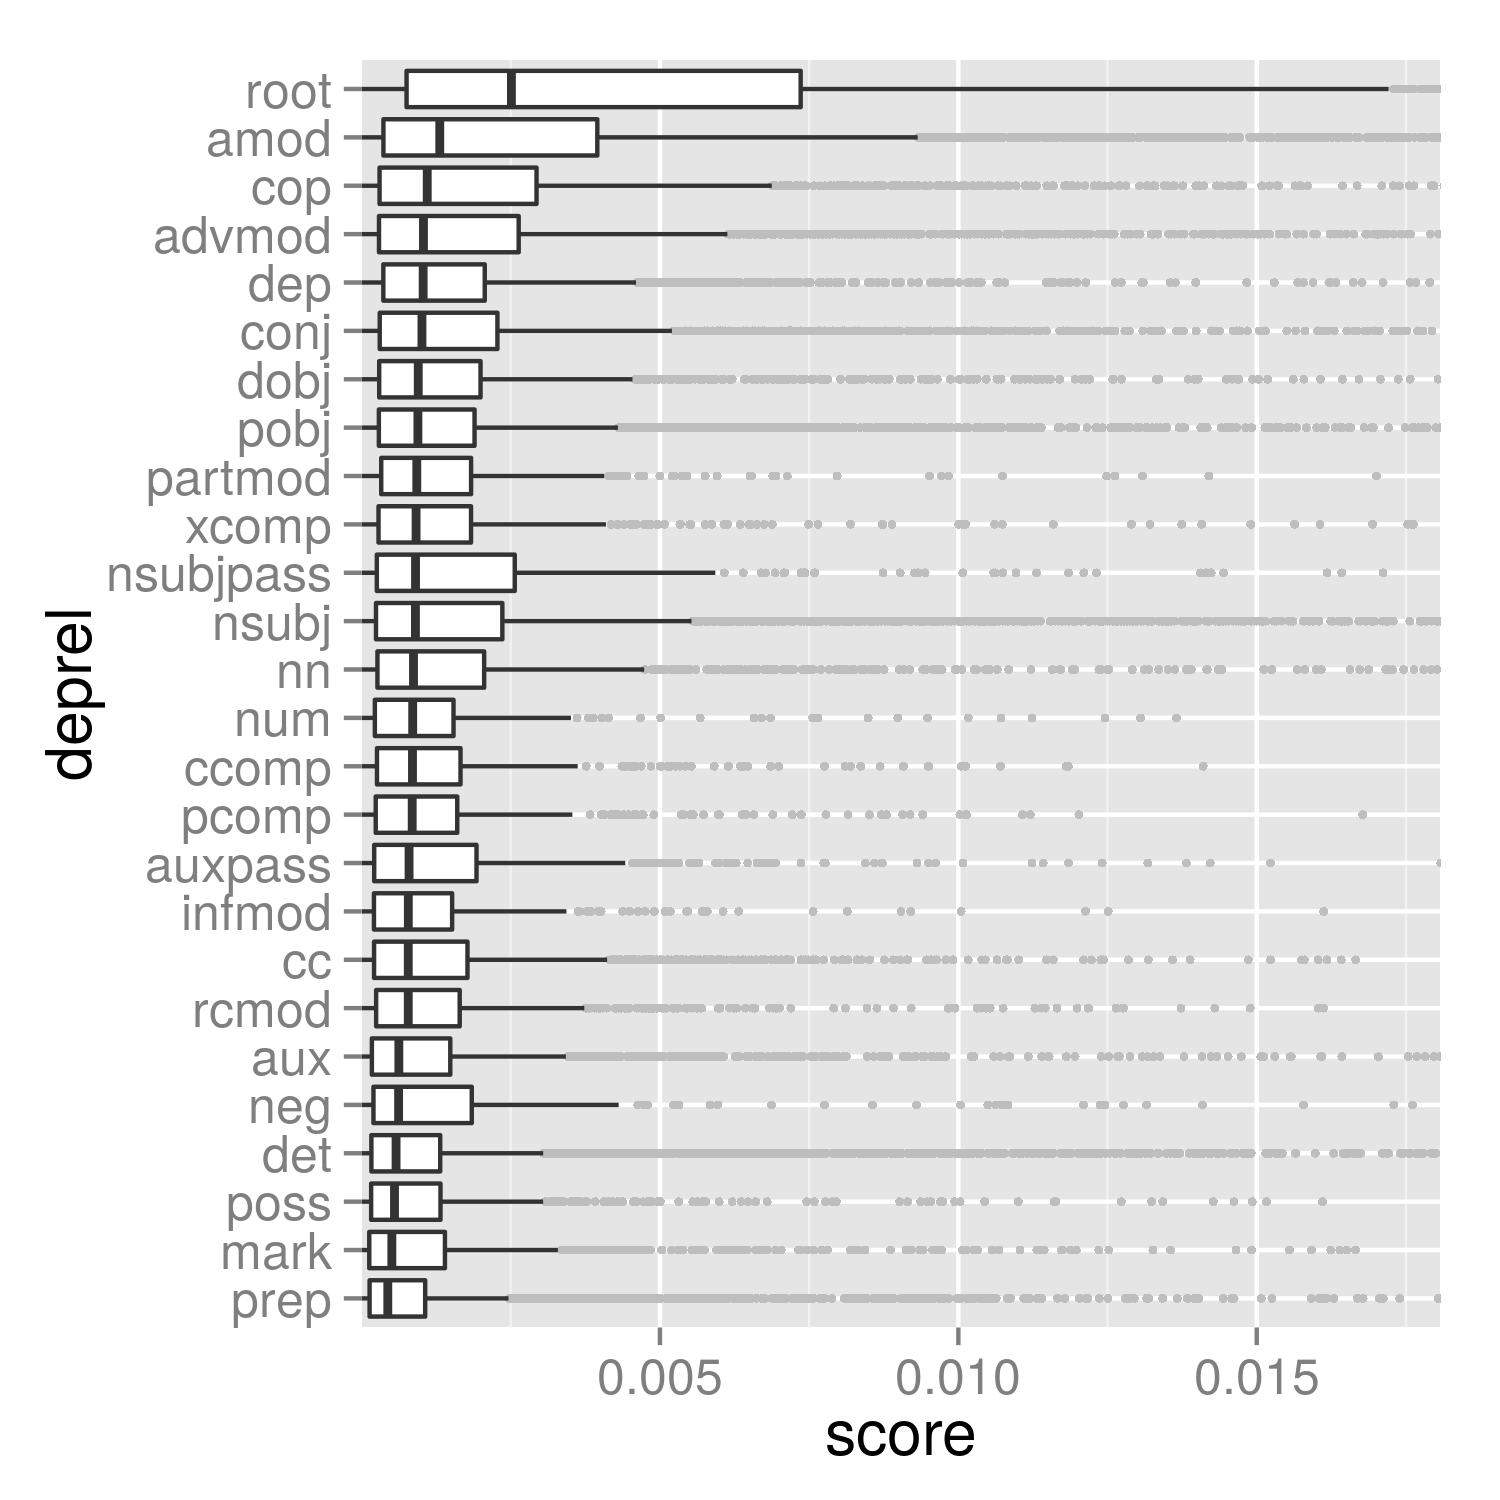
\includegraphics[scale=0.6]{omission-stat/sent-omission-deprel-boxplot.png} 
 %   \caption{Distributions of omission scores per POS category (left)
 %     and dependency relation (right) for {\sc Sentiment}. Only labels
 %   which occurred at least 300 times are included.}
%\label{fig:omission-sent}
%\end{figure*}

%\subsubsection{Omission results for {\sc Sentiment}}
%\label{sec:omitsentiment}
%Figure~\ref{fig:omission-sent} shows the distribution of the omission scores per category for the {\sc Sentiment} model. Superlative adjectives (JJS) such as {\it best, least, scaries} and {\it funniest} are by far the most influential POS category, followed by Adjectives (JJ), Verbs (VBZ, VBG), Nouns (NN, NNS) and Adverbs (RB). Similarly, tokens with function {\sc root} (various verbs, nouns or adjectives central to the meaning of the sentence) are recognized by the model as the most important category, followed by adjectival modifier {\sc amod}. These results support the validity of $\mathrm{omission}$ as a measure of saliency and provide evidence that {\sc Sentiment} learns representations that enable the model to successfully filter out irrelevant parts of the input. 

%-----------------
\label{subsec:omission-text-vis}
\begin{figure}[!htbp]
\centering
%\hspace*{-0.3in}
%\setlength{\tabcolsep}{0pt}
%  \begin{tabular}{cc}
  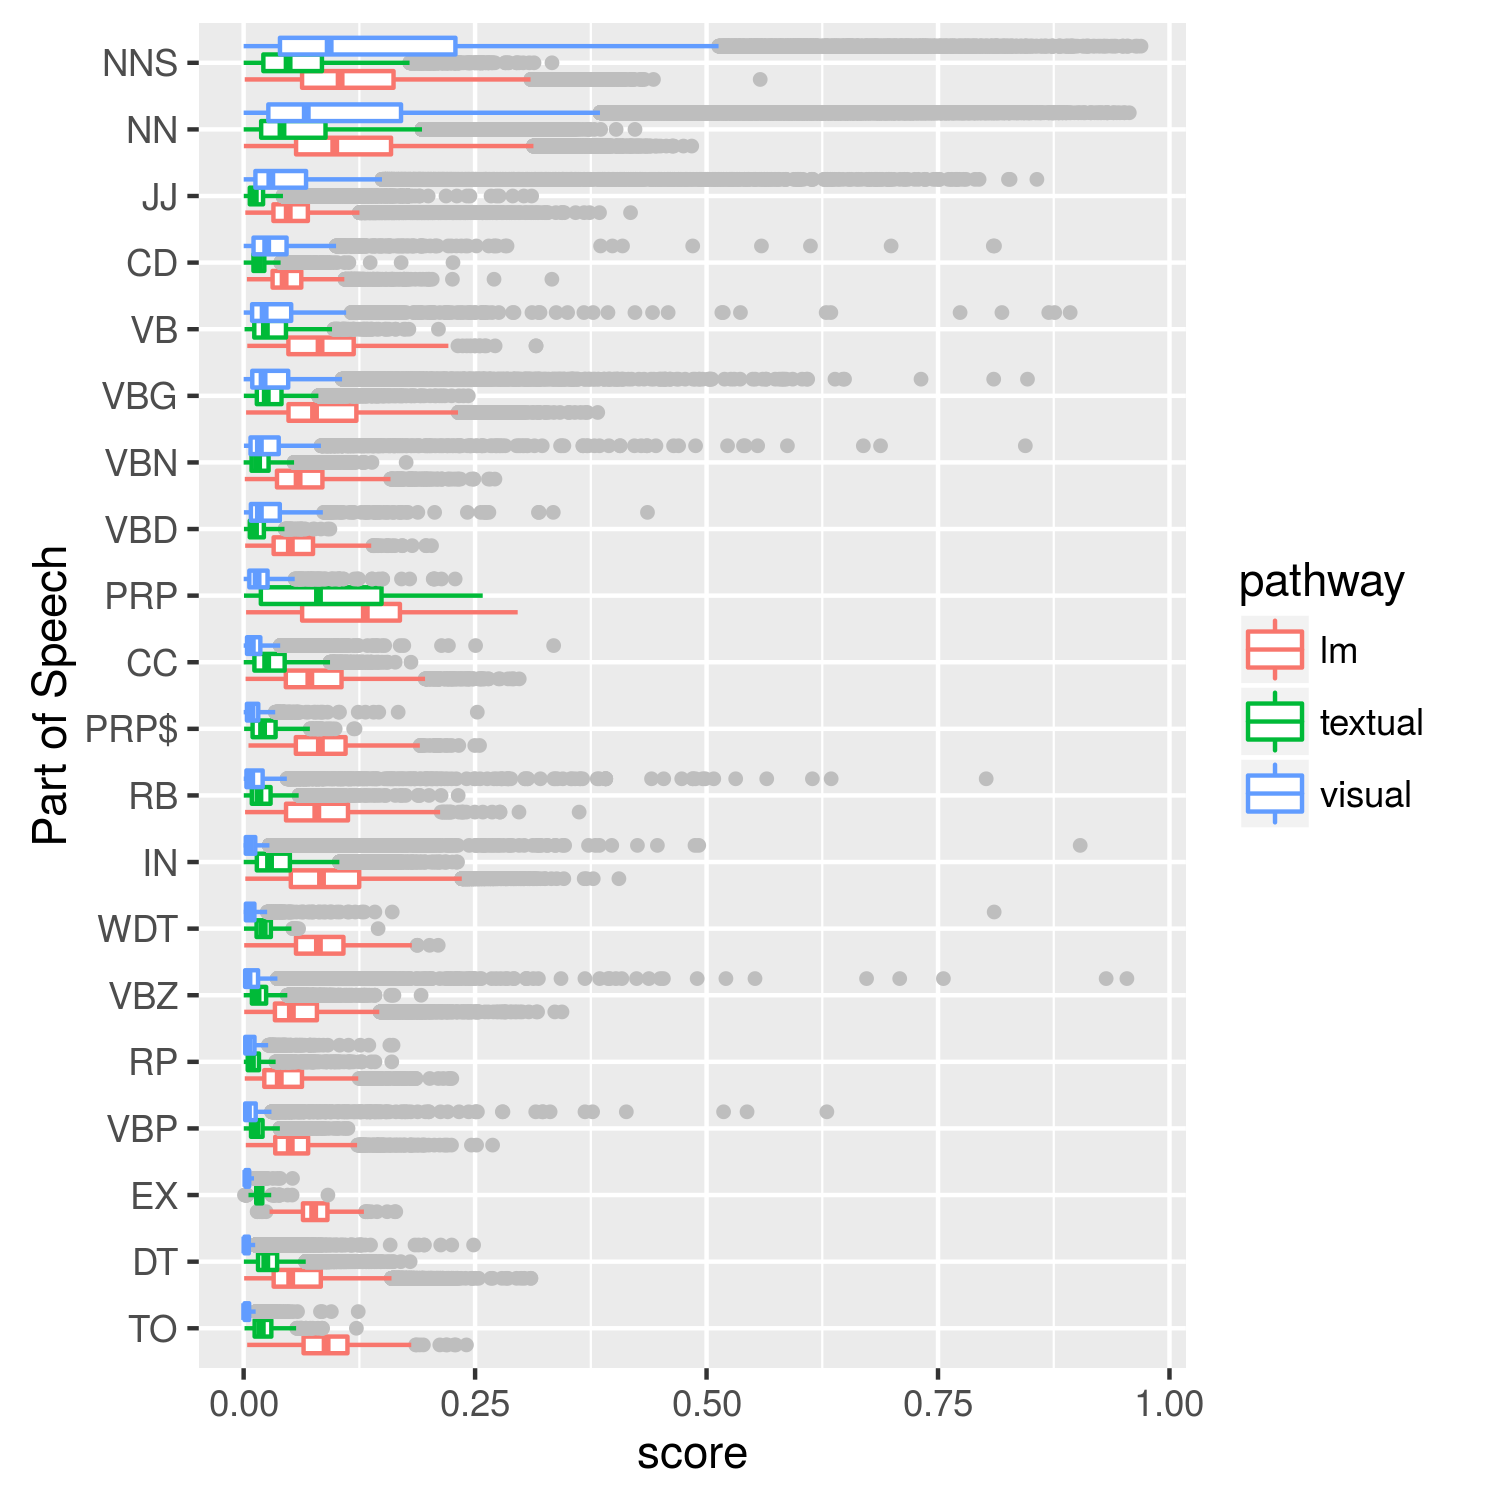
\includegraphics[scale=0.9]{imaginet-omission-pos-boxplot.png} 

  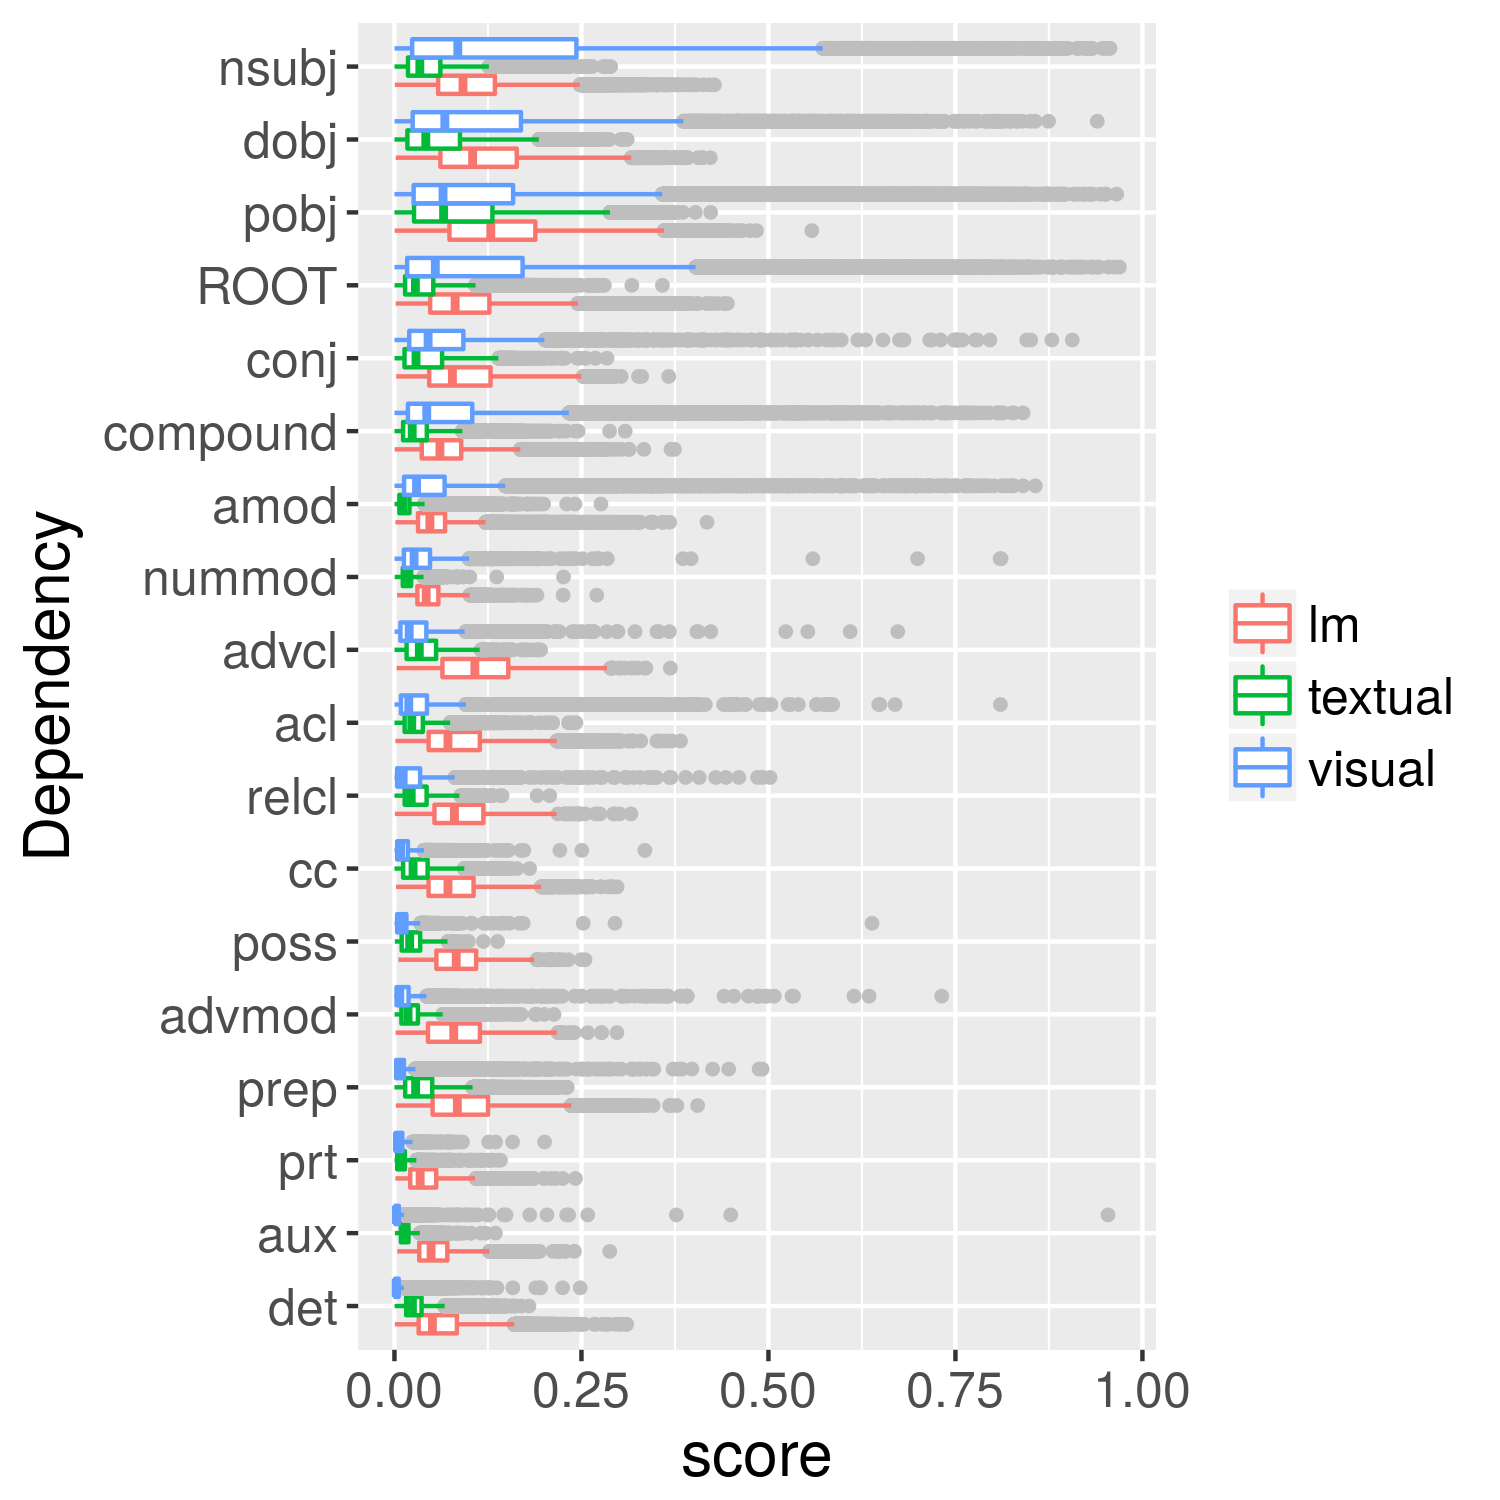
\includegraphics[scale=0.9]{imaginet-omission-dep-boxplot.png} 
%  \end{tabular}
  
\caption{Distribution of omission scores for POS (left) and dependency labels
  (right), for the {\sc Textual} and {\sc Visual} pathways and for
  {\sc LM}. Only labels which occur at least 1250 times are included.}
\label{fig:omission-imaginet}
\end{figure}

\begin{figure*}[t]
  \centering
  \hspace*{-0.2in}
  \setlength{\tabcolsep}{0pt}
  \begin{tabular}{cc}
  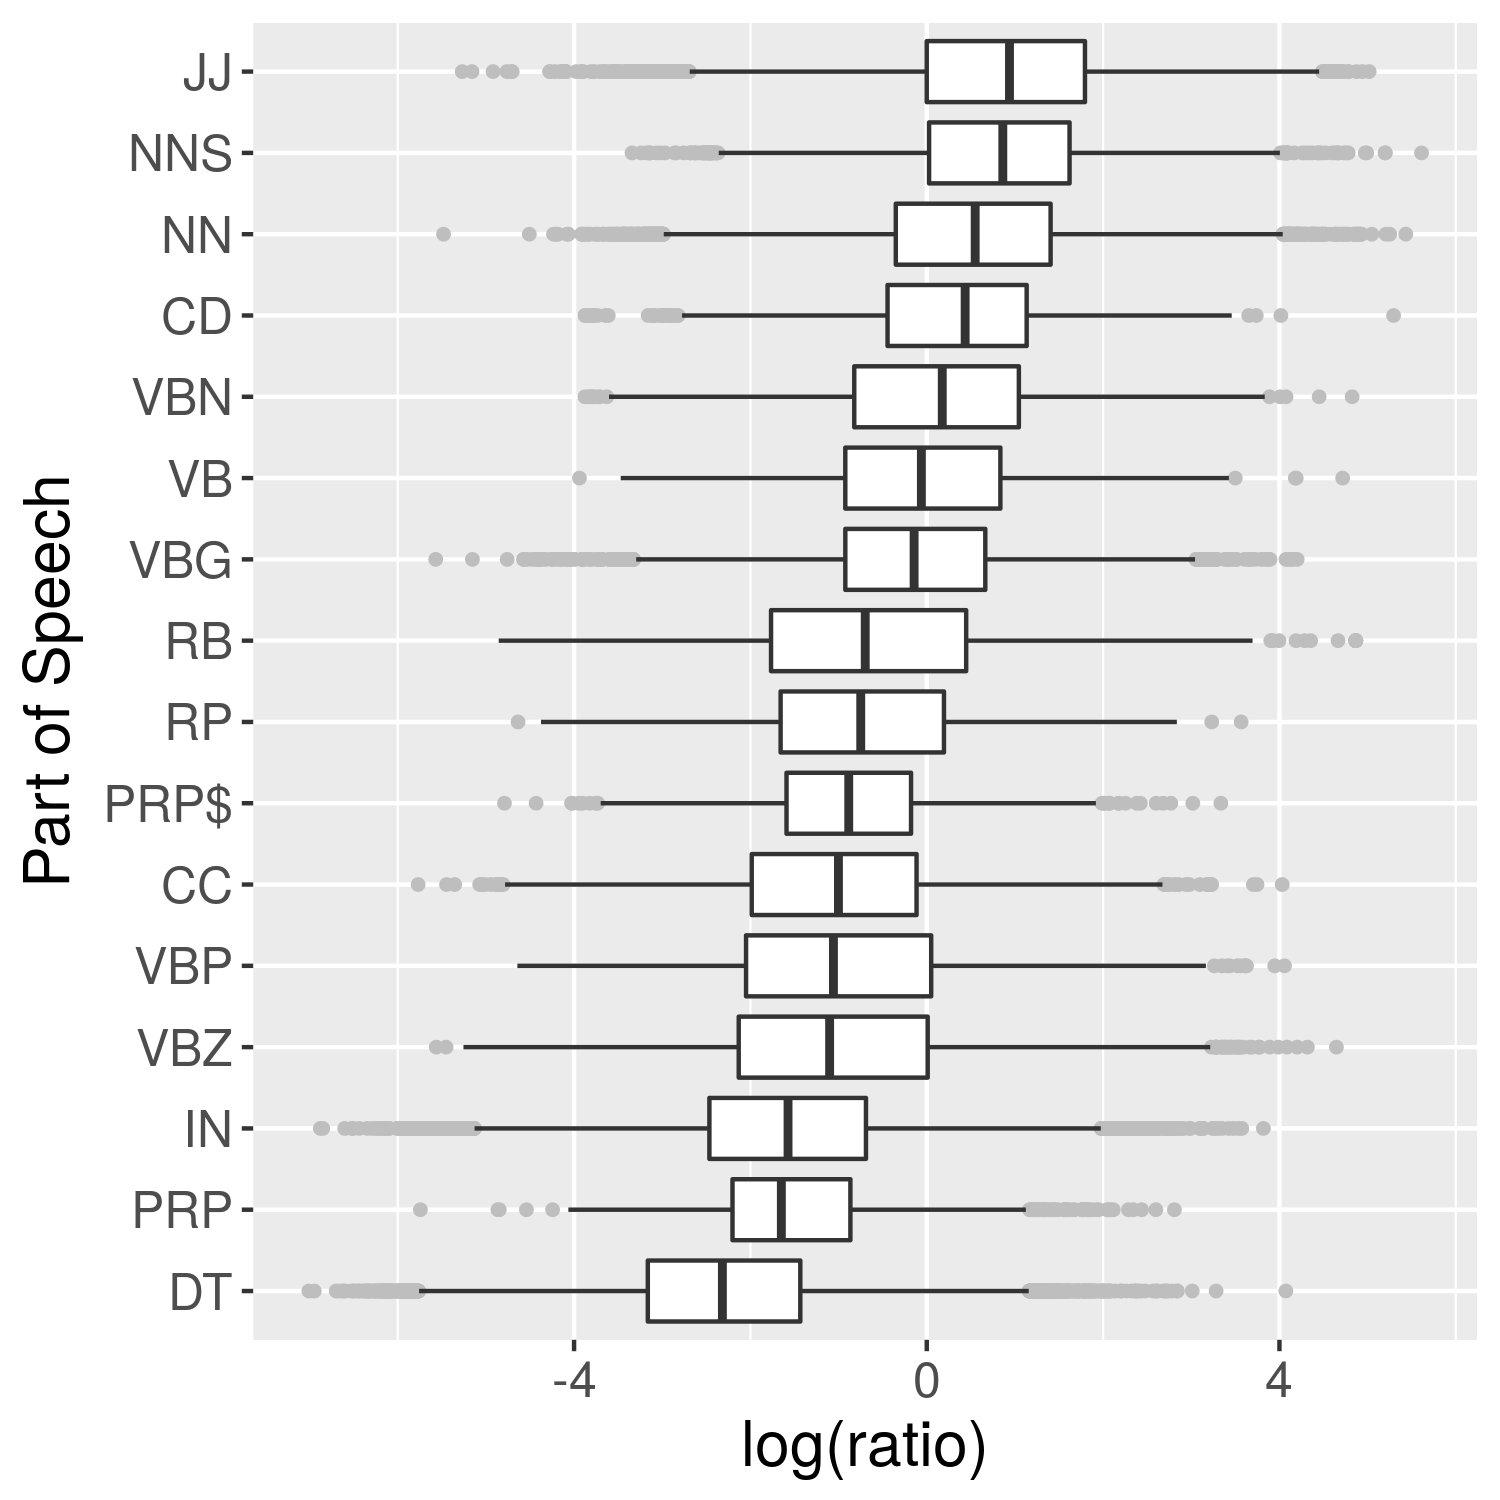
\includegraphics[scale=0.55]{imaginet-omission-ratio-pos-boxplot.png} &
  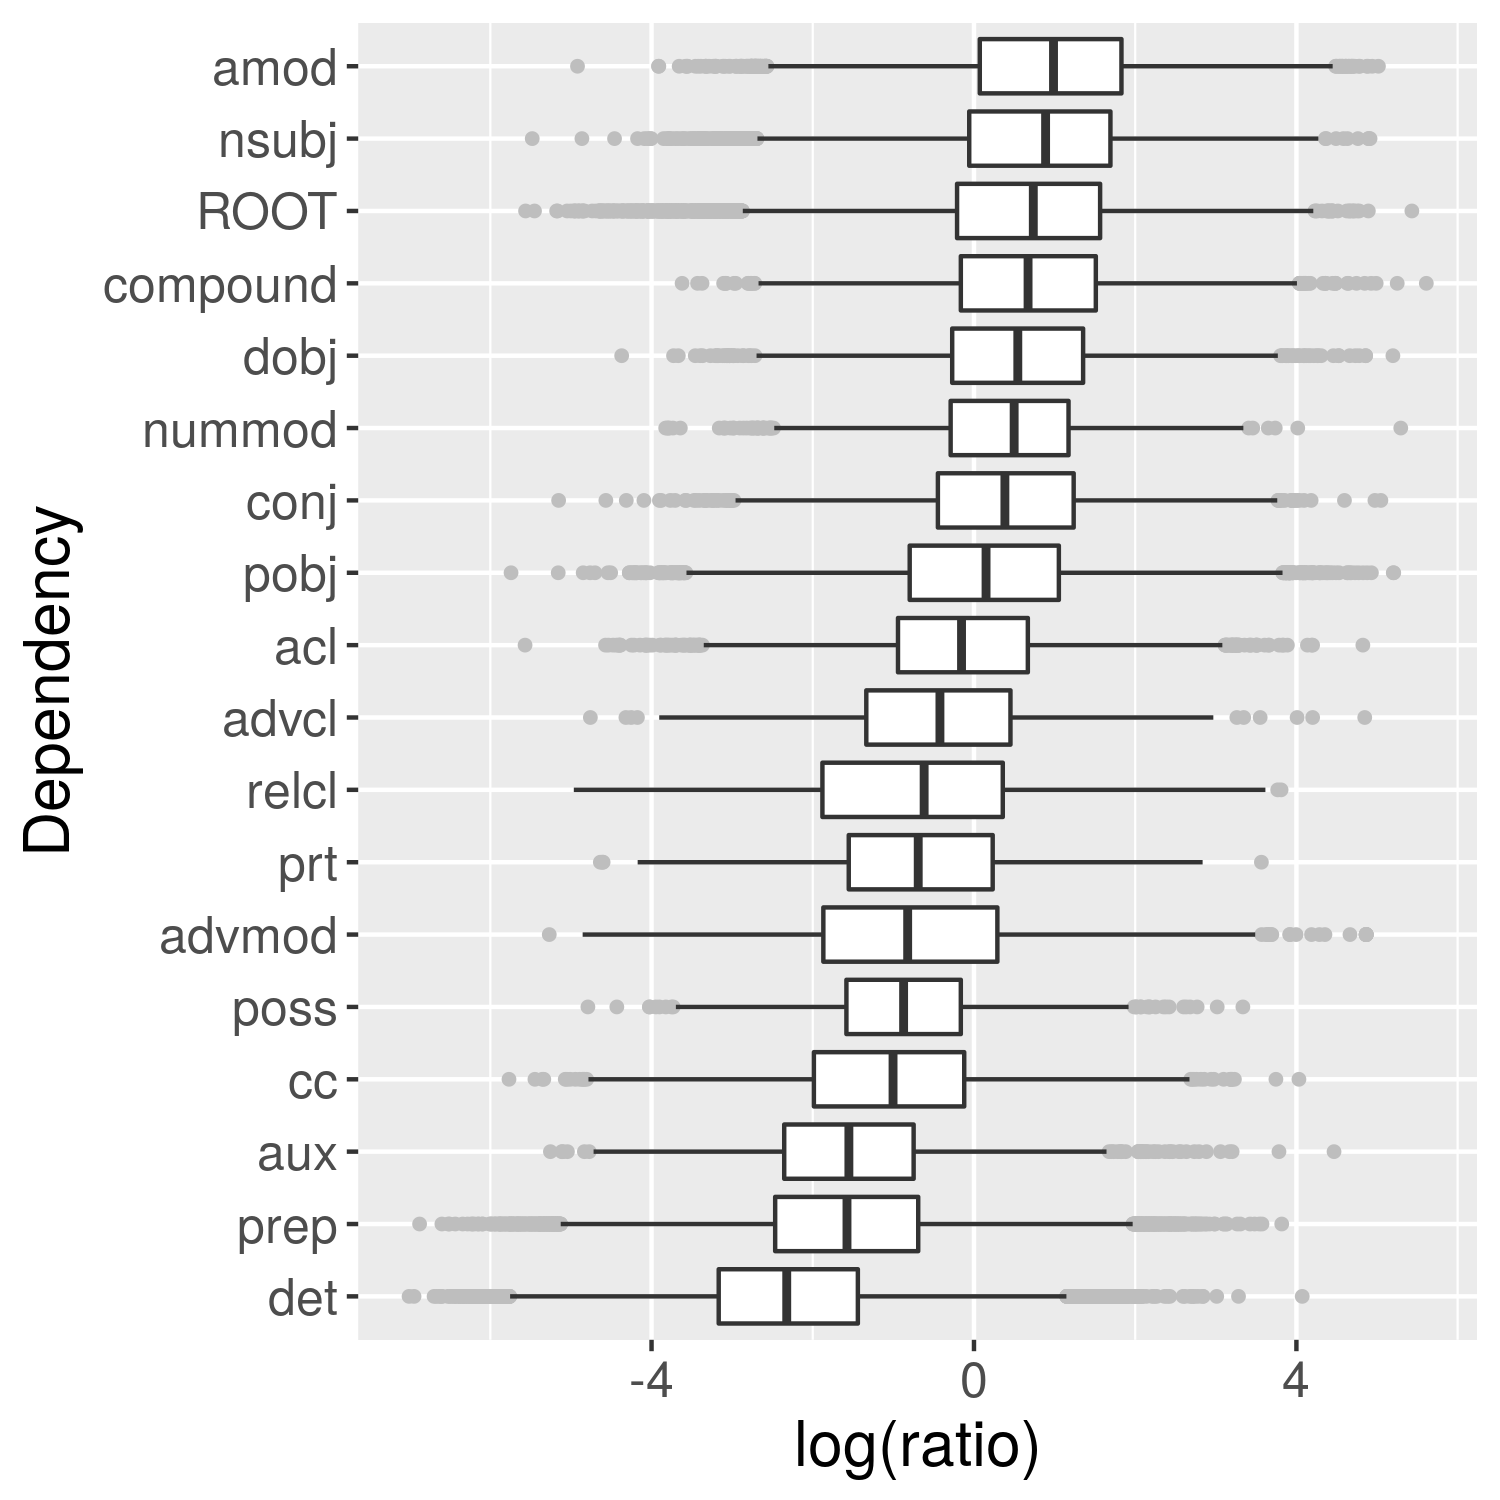
\includegraphics[scale=0.55]{imaginet-omission-ratio-dep-boxplot.png} \\  
  \end{tabular}
  \caption{Distributions of log ratios of omission scores of {\sc Textual} to {\sc Visual} per
    POS (left) and dependency labels (right). Only labels which occur at least 1250 times are included.}
\label{fig:omission-imaginet-ratio}
\end{figure*}



The omission scores can be used not only to
estimate the importance of individual words, but also of syntactic
categories. We estimate the salience of each syntactic category by
accumulating the omission scores for all words in that category. We
tag every word in a sentence with the part-of-speech (POS) category
and the dependency relation (deprel) label of its incoming arc. For
example, for the sentence \emph{the black dog}, we get ({\it
  the},~DT,~det), 
({\it black},~JJ,~amod), ({\it dog},~NN,~root). 
Both POS tagging and dependency parsing are performed 
using the  \verb+en_core_web_md+ dependency parser from the Spacy package.\footnote{Available at
  \url{https://spacy.io/}.} 
%The POS tags used are the Penn Treebank tags and the dependencies are 
%the Stanford basic dependencies.


Figure~\ref{fig:omission-imaginet} shows the distribution of omission
scores per POS and dependency label for the two pathways of {\sc
  Imaginet} and for {\sc LM}.\footnote{The boxplots in this and
  subsequent figures are Tukey boxplots and should be interpreted as follows: the box extends
from the 25th to the 75th percentile of the data; the line across the
box is the 50th percentile, while the whiskers extend past the lower
and upper quartile to $1.5\times$
the interquartile range (i.e.\ 75th percentile - 25th percentile); the
points are outliers.\label{ft:boxplots}}  The general trend is that for the {\sc
  Visual} pathway, the omission scores are high for a small subset of
labels - corresponding mostly to nouns, less so for adjectives and
even less for verbs - and low for the rest (mostly function words and
various types of verbs). For {\sc Textual} the differences
are \label{edit:textualomission} smaller, and the pathway seems to be
sensitive to the omission of most types of words.  For {\sc LM} the
distribution over categories is also relatively uniform, but the omission scores are higher
overall than for {\sc Textual}.

Figure~\ref{fig:omission-imaginet-ratio} compares the two pathways of
{\sc Imaginet} directly using the log of the ratio of the {\sc Visual}
to {\sc Textual} omission scores, and plots the distribution of this
ratio for different POS and dependency labels.  Log ratios above zero
indicate stronger association with the {\sc Visual} pathway and below
zero with the {\sc Textual} pathway. We see that in relative terms,
{\sc Visual} is more sensitive to adjectives (JJ), nouns (NNS, NN),
numerals (CD) and participles (VBN), and {\sc Textual} to determiners
(DT), pronouns (PRP), prepositions (IN) as well finite verbs
(VBZ, VBP).

This picture is complemented by the analysis of the
relative importance of dependency relations: {\sc Visual} pays most
attention to the relations {\sc amod, nsubj, root,
  compound, dobj, nummod}
whereas {\sc Textual} is more sensitive to {\sc det, prep, aux, cc, poss, advmod, prt, relcl}.
As expected, {\sc Visual} is more focused on grammatical
functions typically filled by semantically contentful words, while
{\sc Textual} distributes its attention more uniformly and 
attends relatively more to purely grammatical functions. 

It is worth noting, however, the relatively low omission scores for verbs in case \label{edit:generality}
of {\sc Visual}. One might expect that the task of image prediction from
descriptions requires general language understanding and so high omission
scores for all content words in general, however, the results
suggest that this setting is not optimal for learning useful representations of verbs,
which possibly leads to representations that are too task-specific 
and not transferable across tasks. 

\begin{figure*}[t]
  \centering
  \hspace*{-0.2in}
  \setlength{\tabcolsep}{0pt}
  \begin{tabular}{cc}
  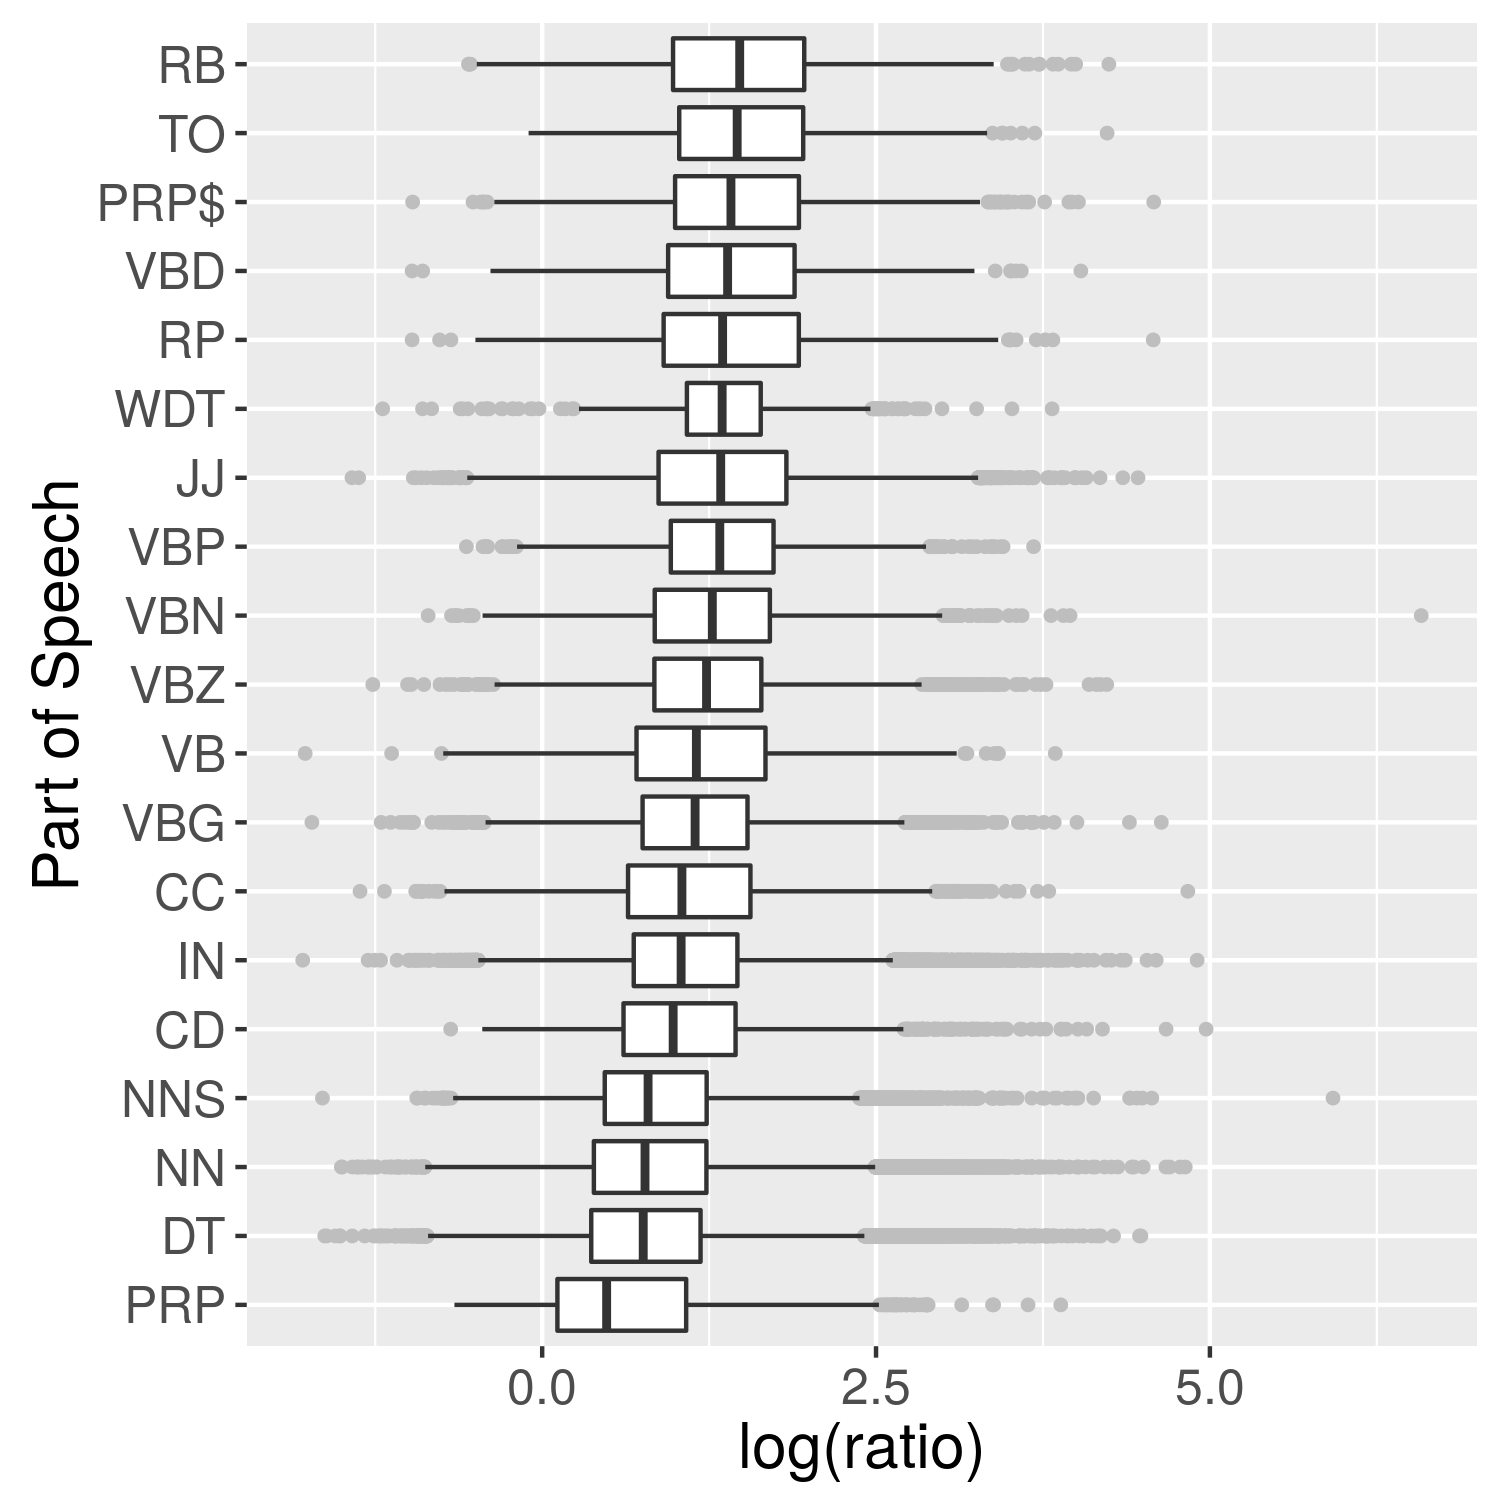
\includegraphics[scale=0.55]{imaginet-omission-quotient-pos-boxplot.png} &
  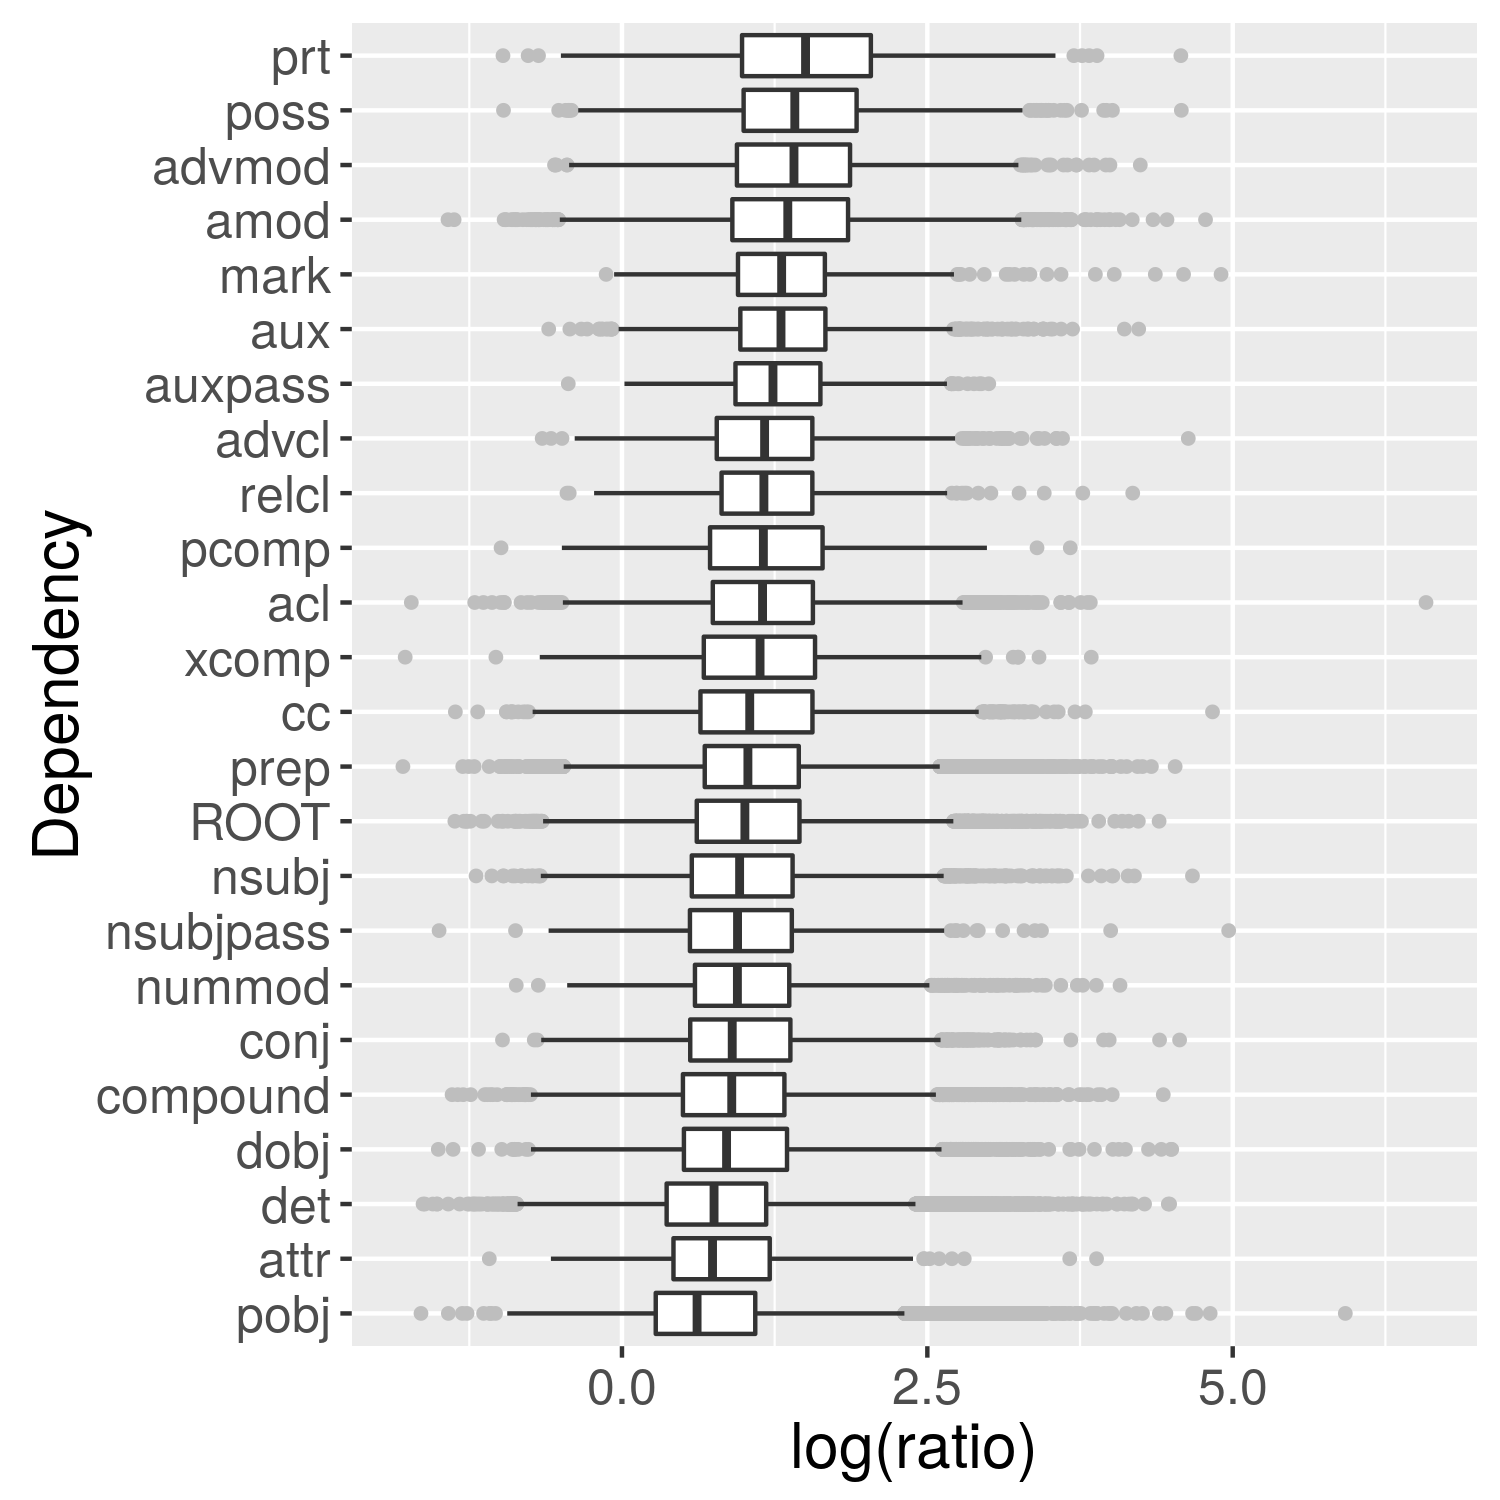
\includegraphics[scale=0.55]{imaginet-omission-quotient-dep-boxplot.png} \\  
  \end{tabular}
  \caption{Distributions of log ratios of omission scores of {\sc LM} to {\sc Textual} per
    POS (left) and dependency labels (right). Only labels which occur at least 1250times are included.}
\label{fig:omission-imaginet-quotient}
\end{figure*}


Figure~\ref{fig:omission-imaginet-quotient} shows a similar analysis
contrasting {\sc LM} with the {\sc Textual} pathway of {\sc
  Imaginet}. The first observation is that the range of values of the
log ratios is narrow, indicating that the differences between these
two networks regarding which grammatical categories they are sensitive
to is less pronounced than when comparing {\sc Visual} to {\sc
  Textual}. While the size of the effect is weak, there also seems to
be a tendency for the {\sc Textual} model to pay relatively more
attention to content and less to function words, compared to
{\sc LM}: it may be that the {\sc Visual} pathway pulls {\sc Textual}
in this direction by sharing word embeddings with it.


Most of our findings up to this point conform reasonably well to prior
expectations about effects that  particular learning objectives should
have. This fact serves to validate our methods. In the next section we
go on to investigate less straightforward patterns.

%The results on syntactic categories for {\sc Visual} are somewhat similar to 
%{\sc Sentiment} in that both models seem to learn to focus on one
%particular category (Nouns for {\sc Visual}, Adjectives for {\sc Sentiment}). 
%{\sc Visual} still incorporates adjectives, personal
%pronouns and verbs to the representations, but tends to ignore
%words of other categories. 


\subsection{Beyond Lexical Cues}
\label{sec:beyondlexical}

Models that utilize the sequential structure of language 
have the capacity to interpret the same word-type differently depending on
the context. The omission score distributions in Section \ref{sec:omitimaginet} 
show that in the case of {\sc Imaginet} the 
pathways are differentially sensitive to content vs.\ function
words. In principle, this may be either just due to purely lexical features or the model 
may actually learn to pay more attention to the same word type in appropriate
contexts. This section investigates to what extent our models
discriminate between occurrences of a given word in different positions and 
grammatical functions. 


%The analysis we described here takes
%the omission scores as input data, therefore it can be potentially applied 
%to any architecture for which the omission scores can be computed. However,
%the presented analysis and results regarding word positions can only be meaningful
%for Recurrent Neural Networks as they compute their representations sequentially and are not
%limited by fixed window sizes.\footnote{CNNs with multi-word filters
%and tree-structured recursive neural networks do not incrementally build representations
%of sentences in a left-to-right or right-to-left fashion. 
%Bi-directional RNNs, on the other hand, are sensitive by word-order and can potentially
%learn to handle the same word in different positions differently. \label{edit:foot}}

We fit four L2-penalized linear regression models which predict the omission 
scores per token with the following predictor variables: 
\begin{enumerate}
	\item {\sc LR word}: word type
	\item {\sc LR +dep}: word type, dependency label and their interaction 
	\item {\sc LR +pos}: word type, position (binned as {\sc first, second, third, middle,
	antepenult, penult, last}) and their interaction
	\item {\sc LR full}: word type, dependency label, position, word:dependency interaction, 
	word:position interaction
\end{enumerate}

\noindent We use the 5000-image portion of MSCOCO validation data for 
training and test. The captions contain about 260,000 words in total, of 
which we use 100,000 to fit the regression models. We then use the rest 
of the words to compute the proportion of variance explained by the models. 
For comparison we also use the {\sc Sum} model which composes word
embeddings via summation, and uses the same loss function as {\sc
  Visual}. This model is unable to encode information about word
order, and thus is a good baseline here as we investigate the
sensitivity of the networks to positional and structural cues.

\begin{table}
  \centering
  \caption{Proportion of variance in omission scores explained by
    linear regression.}
    \begin{tabular}{l|rrrr}
               & word   & +pos  & +dep  & full \\\hline
     {\sc Sum}       & 0.654  & 0.661 & 0.670 & 0.670 \\
     {\sc LM}        & 0.358  & 0.586 & 0.415 & 0.601 \\
     {\sc Textual}   & 0.364  & 0.703 & 0.451 & 0.715 \\
     {\sc Visual}    & 0.490  & 0.506 & 0.515 & 0.523 \\
    \end{tabular}
    \label{tab:lr-r2}
\end{table}


Table~\ref{tab:lr-r2} shows the proportion of variance $R^2$ in omission
scores explained by the linear regression with the different predictors.
The raw $R^2$ scores show that for the language models {\sc LM} and 
{\sc Textual}, the word-type predicts the omission-score to much smaller 
degree compared to {\sc Visual}. Moreover, adding information about 
either the position or the dependency labels increases the explained variance for all models. 
However, for the {\sc Textual} and {\sc LM} models the position of the word adds 
considerable amount of information. This is not surprising considering that the omission
scores are measured with respect to the final activation state, and
given the fact that in a language model the recent history is most
important for accurate prediction.

Figure~\ref{fig:rsquared} offers a different view of the data to, showing
the increase or decrease in $R^2$ for the models relative to {\sc LR~+pos} 
to emphasise the importance of syntactic structure beyond the position in the sentence.
Interestingly, for the {\sc Visual} model, dependency labels are 
more informative than linear position, hinting at the importance of syntactic 
structure beyond linear order. There is a sizeable increase in $R^2$ between 
{\sc LR~+pos} and {\sc LR~full} in the case of {\sc Visual}, suggesting that 
the omission scores for {\sc Visual} depend on the words'
grammatical function in sentences, {\it even after controlling for word
identity and linear position.}  In contrast, adding additional information on
top of lexical features in the case of {\sc Sum} increases the
explained variance only slightly, which is most likely due to the unseen words
in the held out set.   

Overall, when regressing on word identities, word position and
dependency labels, the {\sc Visual} model's omission scores are the
hardest to predict of the four models suggesting that the model may be
encoding additional structural features not captured by these predictors. 
We will look more deeply into such potential features in the following sections.

\begin{figure}
\centering
  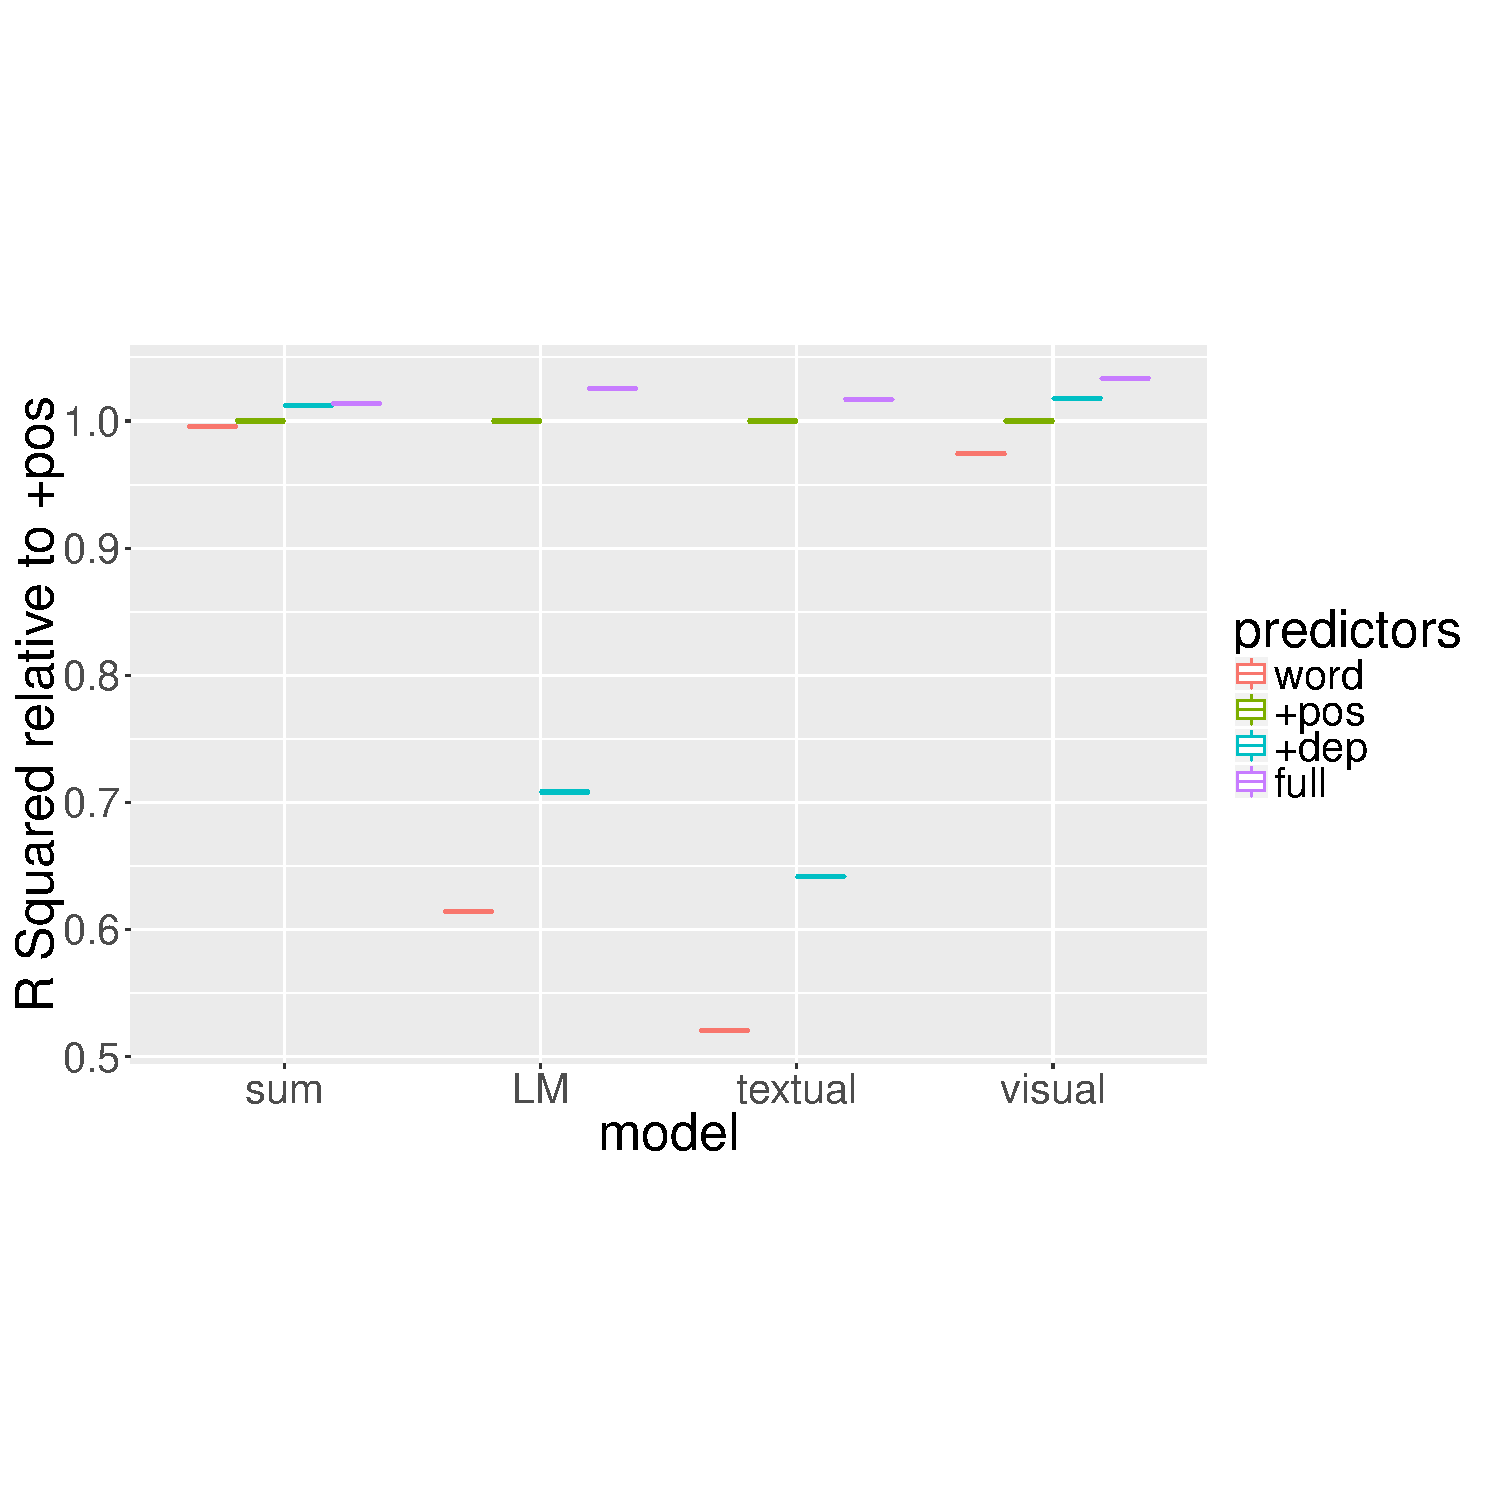
\includegraphics[scale=0.35]{position-new.pdf}
\caption{Proportion of variance in omission scores explained by the
  linear regression models
 for {\sc Sum}, {\sc LM}, {\sc Visual} and {\sc Textual}, relative to
 regressing on word identity and position only. }
\label{fig:rsquared}
\end{figure}


\subsubsection{Sensitivity to grammatical function}
\label{sec:gramfunc}

%\begin{figure}[t]
%  \centering
%  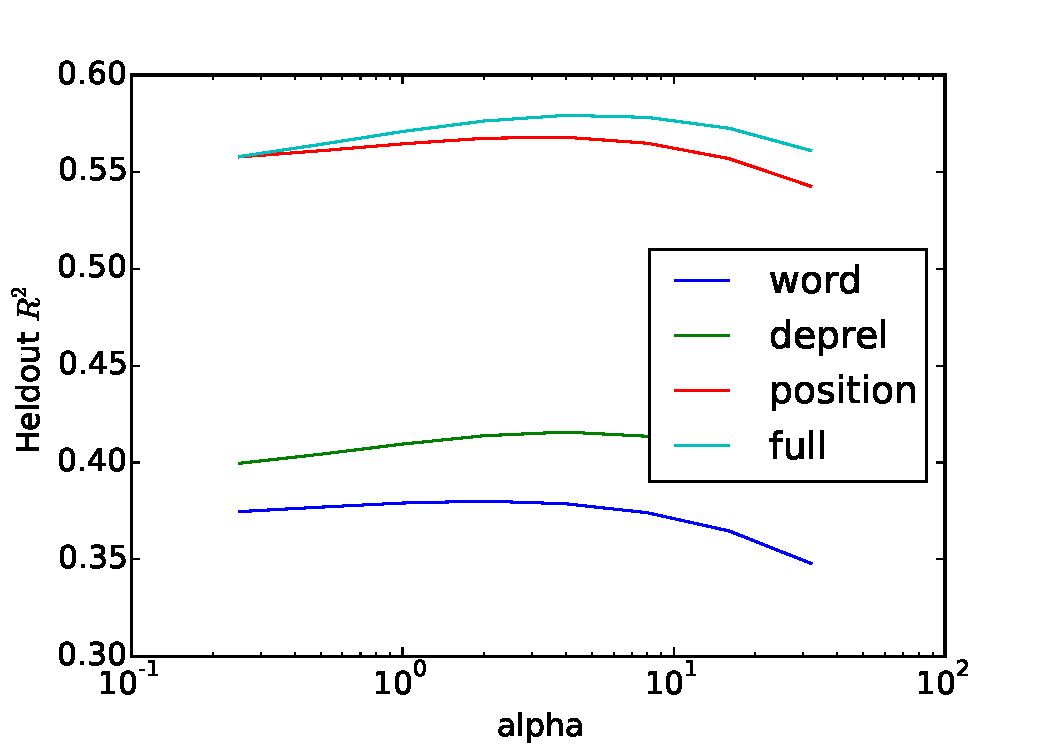
\includegraphics[scale=0.4]{omission-stat/scores-vs-alpha.pdf}
%  \caption{Proportion of variance in omission scores explained by {\sc Model 1} vs {\sc Model 2} as a function of regularization parameter $\alpha$.}
%  \label{fig:scores-vs-alpha}
%\end{figure}

\begin{figure}[t]
  \centering
  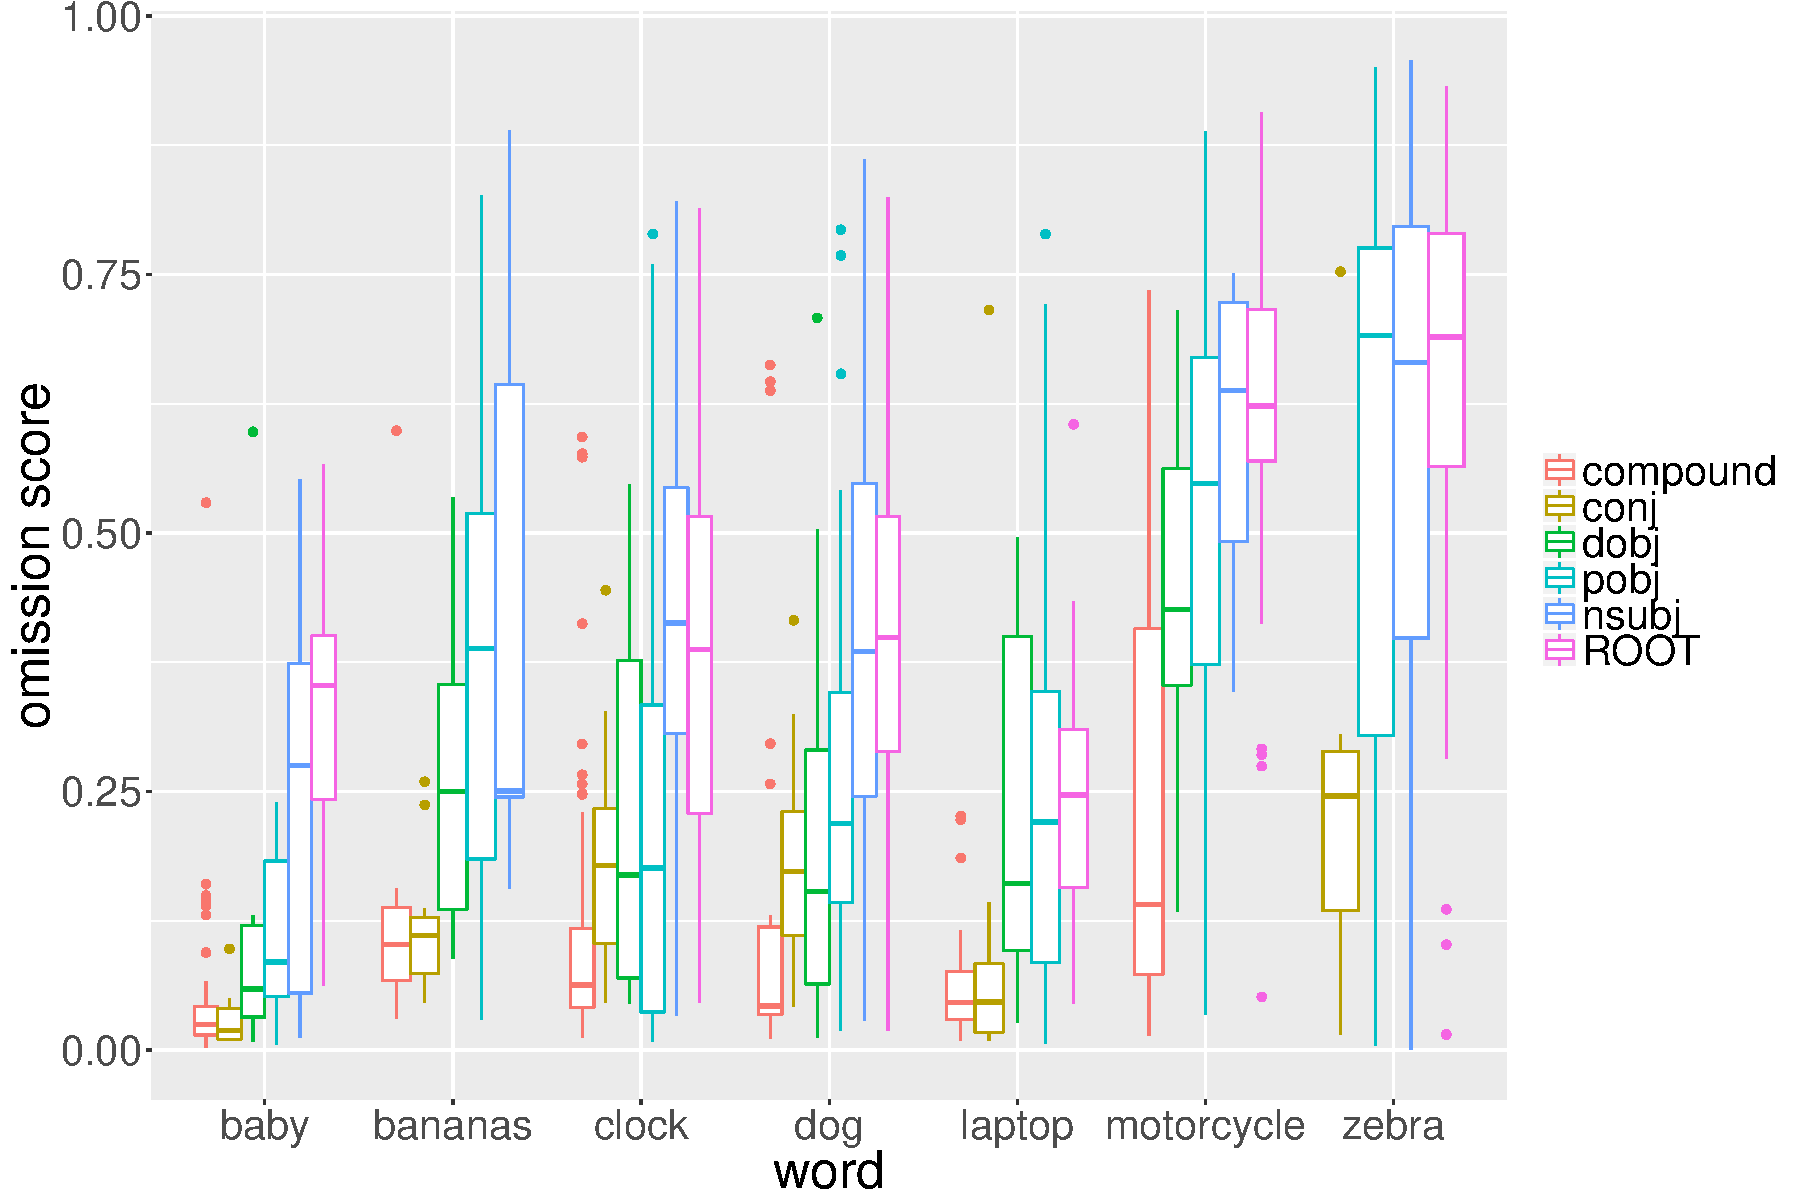
\includegraphics[scale=0.35]{top_words.pdf}
  \caption{Distribution of omission scores per deprel label for the selected word types.}
  \label{fig:top_words}
\end{figure}
%\todo{At some point redo this with words ranked by ratio between the errors not the difference}

In order to find out some of the specific syntactic configurations leading to
an increase in $R^2$ between the {\sc LR~word} and {\sc LR~+dep} predictors
in the case of {\sc Visual}, we next considered all word types with
occurrence counts of at least 100 and ranked them according to how much
better, on average, {\sc LR~+dep} predicted their omission scores 
compared to {\sc LM~word}. 

Figure~\ref{fig:top_words} shows the per-dependency 
omission score distributions for seven top-ranked words.
There are clear and large differences in how these words
impact the network's representation depending on what grammatical
function they fulfill. They all have large omission scores when they
occur as {\sc nsubj} (nominal subject) or {\sc root}, likely due to the fact that these
grammatical functions typically have a large contribution to the
complete meaning of a sentence.  Conversely, all have small omission 
scores when appearing as {\sc conj} (conjunct): this is probably because in this position
they share their contribution with the first, often more important,
member of the conjunction, for example in {\it A cow and its baby eating
  grass}. 
% The pattern for {\sc nn} (nominal modifier) is a bit more complicated: for
% four of the words shown (as well as for most other words not shown in
% the figure), the score is very low in this grammatical function--presumably 
% because most words contribute less to the sentence meaning when used  
% as modifiers than as heads (e.g.\ {\it a clock tower}). However,
% for the words {\it zebra} and {\it water}, omission scores are high
% when they act as a nominal modifier {\sc nn}. This appears due to two reasons:
% \begin{enumerate}
% \item For {\it zebra}, there are frequent erroneous parses such as {\it
%     zebra/{\sc nn} browsing/{\sc root}} instead of {\it zebra/{\sc nsubj} browsing/{\sc
%     root}}. The network does not make this mistake, and treats these
%     occurrences of {\it zebra} according to its importance as {\sc nsubj}.
% \item {\it Water} as a modifier often changes the meaning of its head in
%  a visually salient way: e.g.\ {\it water fall, water balloon, water scene, water skiing}, and
%   thus the network learns that this particular word is important in the modifier position.
% \end{enumerate}

\subsubsection{Sensitivity to linear structure}
\label{subsec:information-struct}

\begin{figure}
\centering
 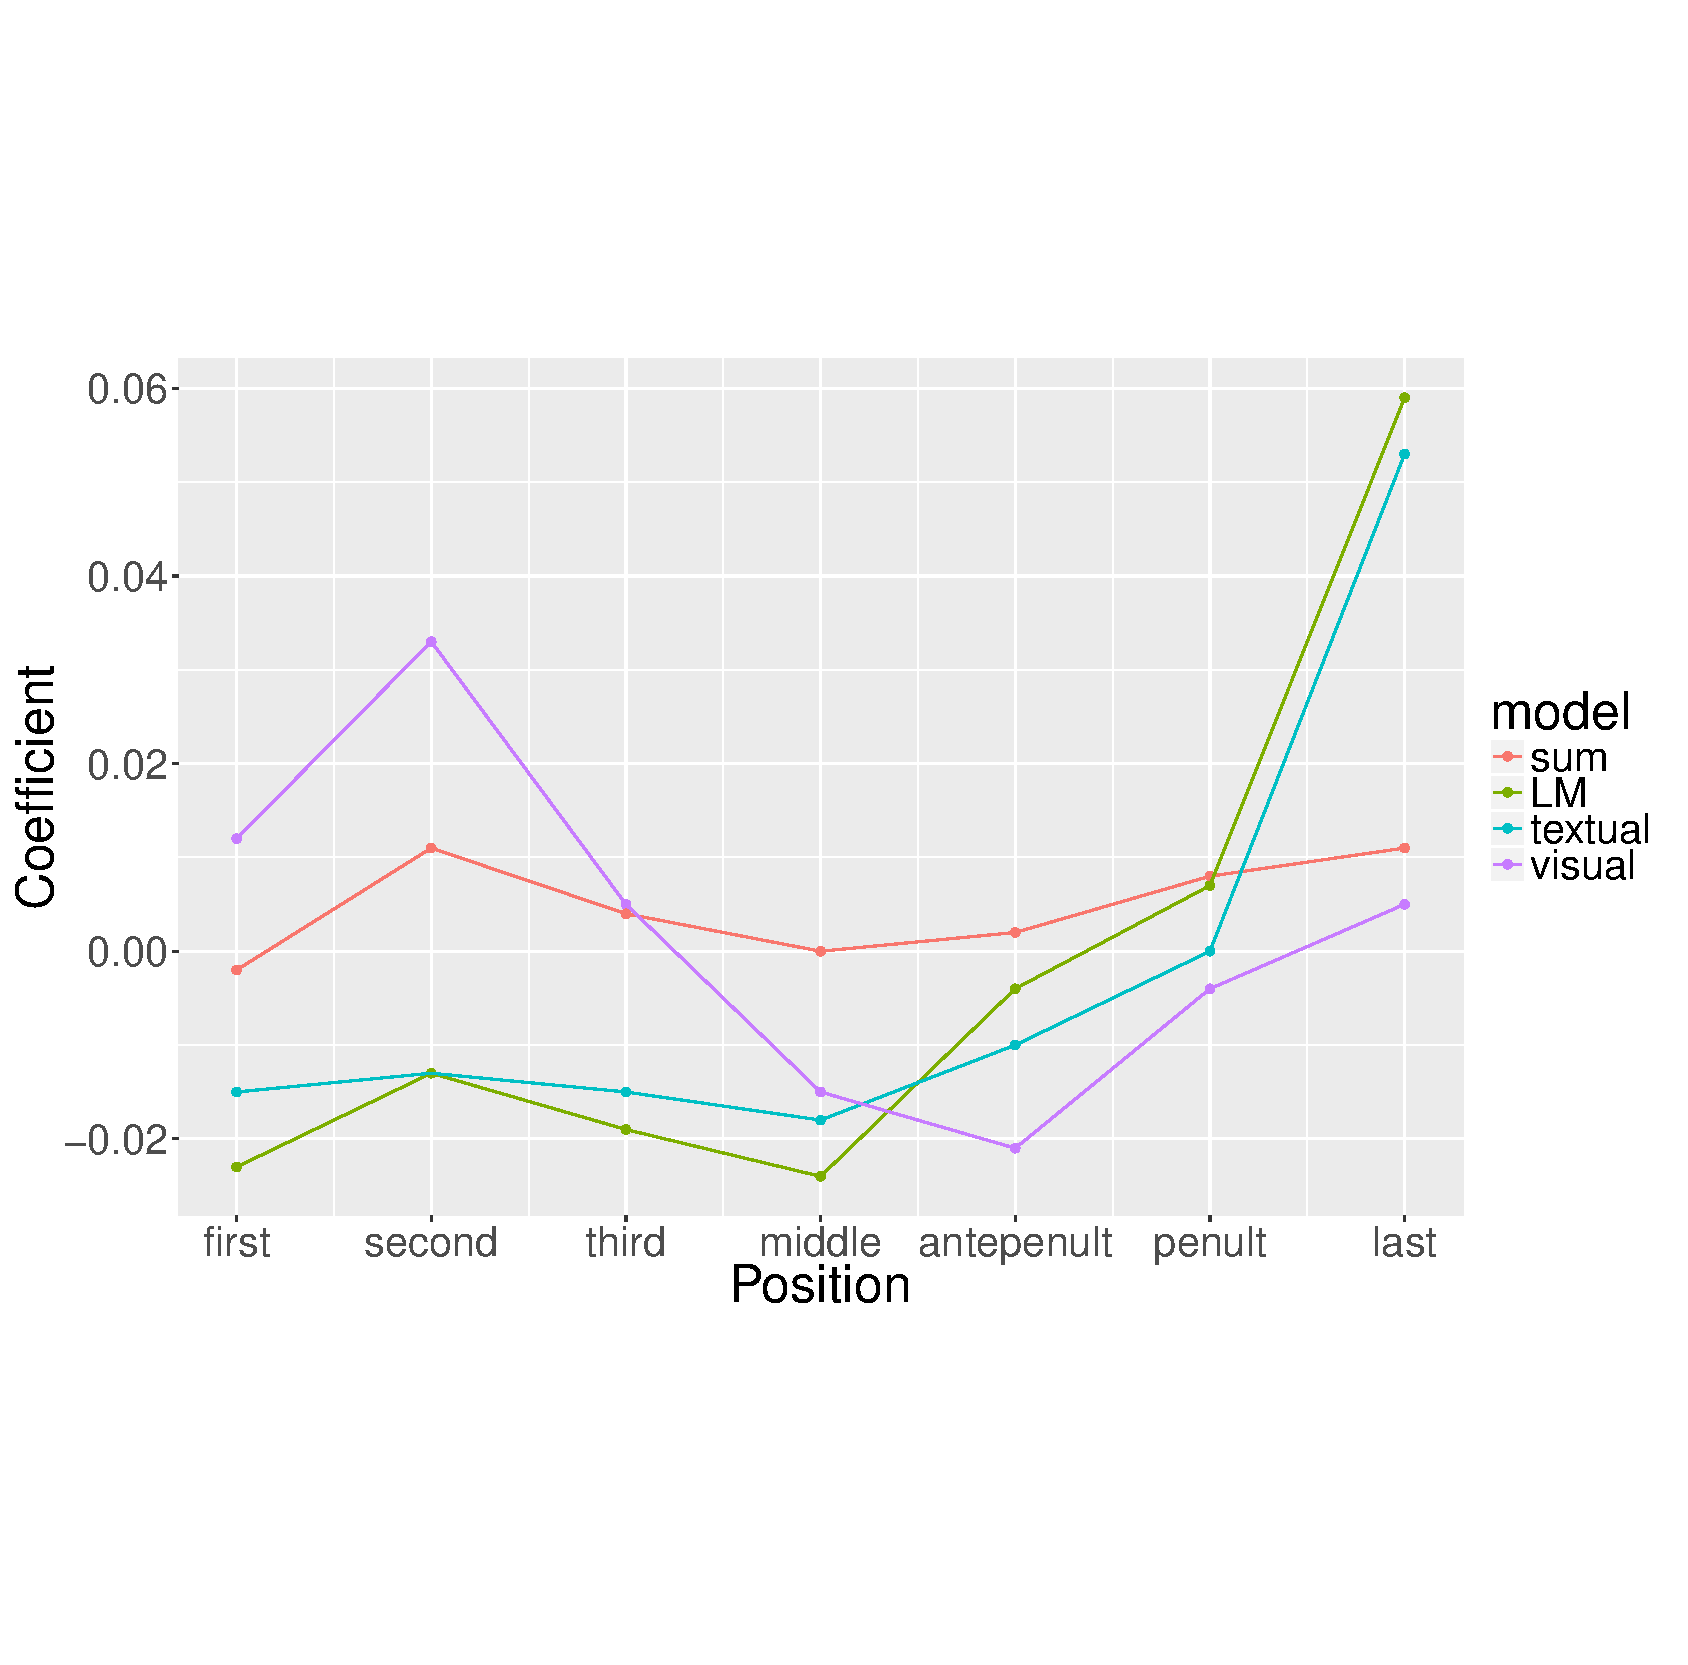
\includegraphics[scale=0.4]{position-coef.pdf}
 \caption{Coefficients on the y-axis of {\sc LR full} corresponding to the
position variables on the x-axis.}
 \label{fig:posrqs}
\end{figure}
 
As observed in Section \ref{sec:beyondlexical}, 
adding extra information about the position of words 
explains more of the variance in the case of {\sc Visual} and especially
{\sc Textual} and {\sc LM}.
Figure \ref{fig:posrqs} shows the coefficients corresponding to the
position variables in {\sc LR~full}. Since the omission scores 
are measured at the end-of-sentence token, the expectation is that 
for {\sc Textual} and {\sc LM}, as language models,  
the words appearing closer to the end of the sentence would have a
stronger effect on the omission scores. This seems to be confirmed by
the plot as the coefficients for these two networks up until the
\emph{antepenult} are all negative. 


For the {\sc Visual} model it is less clear what to
expect: on the one hand due to their chain structure,  
RNNs are better at keeping track of
short-distance rather than long-distance dependencies and thus we can expect 
tokens in positions closer to the end of the sentence to be more important. 
On the other hand in English the information structure of a single
sentence is expressed via linear ordering: the {\sc topic} of a 
sentence appears sentence-initially, and the {\sc comment} follows. 
In the context of other text types such as dialog or multi-sentence \label{edit:topiccomment}
narrative structure, we would expect {\sc comment} to often be more
important than {\sc topic} as {\sc comment} will often 
contain new information in these cases. In our setting of image captions 
however, sentences are not part of larger discourse, it is sentence
initial material that typically contains the most important 
objects depicted in the image, e.g. {\it {\underline{two zebras}} are grazing in tall grass on a savannah.}
Thus, for the task of predicting features of the visual scene, it would 
be advantageous to detect the topic of the sentence and up-weight its
importance in the final meaning representation. Figure \ref{fig:posrqs}
appears to support this hypothesis and the network does 
learn to pay more attention to  words appearing
sentence-initially. This effect seems to be to some extent mixed with the recency
bias of RNNs as perhaps indicated by the relatively high coefficient of the {\it last}
position for {\sc Visual}. 


% The basic idea is to focus on
% words which occur in several grammatical functions, and see whether
% the network treats the different occurrences differently based on the
% dependency label. 

% The omission score results for {\sc Visual}
% suggest that the model pays relatively more attention to 
% categories {\sc nsubj, pobj, root} than to {\sc nn}. 
% Since the same word types can potentially
% assume these categories in different contexts which leads to the
% hypothesis that {\sc Visual} learned to recognize small syntactic 
% constructions. In the following experiment we consider word types 
% that appear with all four of the following dependency labels: 
% {\sc nsubj, pobj, root, nn}. Table \ref{tab:nnexample} demonstrates
% examples of the systematic pattern that in when tokens with deprel {\sc nn}
% have the lowest 

% A systematic pattern that provides evidence to support
% the hypothesis is that when nouns assume the role of noun complement
% {\sc nn}, their omission score is the lowest. This result is illustrated
% in 

% \iffalse
% \subsection{Distribution of omission scores}

% Determining feature importances from RNN hidden states for NLP tasks
% allows to uncover what kinds linguistic features models focus on.  We
% showed that omission scores allow for interesting qualitative
% comparison between RNN based models, but also provides insight into
% the nature of the combinations of data sets and tasks. The omission
% score results shows that to estimate the polarity of the sentence a
% model should primarily focus on adjectives. More interestingly the
% relative higher omission scores for Nouns for {\sc Visual} suggests
% that combination of the MS-COCO data set and the pre-trained VGG-CNN
% image-representation prediction as objective does not seem to promote
% the model to learn to pay attention to verbs. This analysis suggests
% that this particular setting does not allow the model to learn general
% representations for phrases/sentences as it promotes filtering out the
% information content of verbs.  Relative to {\sc Visual} the
% omission-score distribution of the {\sc Skip-gram} is much flatter
% providing an indication that the model does not throw away as much
% important linguistic information.  \todo{show some plot of the
%   distributions VISUAL vs. skip-gram} \fi

%\section{Analysis of the function of individual hidden units}
%\label{sec:micro}
%
%\subsection{Top $K$ contexts}
%\label{sec:topk}
%
%\begin{table}[t]
%\small
%\caption{Contexts from the top 20 trigrams for example hidden units in each pathway.}
%\label{tab:contexts}
%\vspace{.2cm}
%\centering
%    \begin{tabular}{ | p{6cm} | p{6cm}|}
%    \hline
%    {\sc Visual} & {\sc Textual} \\
%    \hline
%   examples & examples  \\
%   \hline
%   \end{tabular}
%\end{table}
%
%
%The aim of this section is to develop methods that allow
%for the qualitative analysis of the kinds of linguistic features
%that individual hidden dimensions of RNNs encode. 
%We develop a simple method we dub {\it top $K$ contexts} 
%after the {\it top $K$ images} of \namecite{zhou2014object}.
%In this technique, we forward each sentence
%token by token through an RNN, and register the activation 
%of each unit in the last hidden layer of the network $\mathbf{h}_{t}$
%at each time step $t$. This results in a vector $M_i$ 
%for each hidden unit $i$, which contains  the activation of that unit 
%as a response to every token in the corpus.
%
%For each unit $i$, the entries with the highest absolute values in 
%$M_i$ represent the triggers that unit $i$ is most sensitive to. The 
%triggers could be a single token, or an n-gram including the token 
%received at the time of activation. We call such n-grams {\it top 
%contexts} of unit $i$. In this section, we analyze the top $k$ contexts
%of the hidden units to see whether they share any syntactic and/or 
%semantic patterns, indicating the function each unit is trained to perform.
%We also provide a comparison of the kinds of features the {\sc Visual} and 
%{\sc Textual} pathways of {\sc Imaginet} encode based on analysis on the 
%top $K$ contexts from the validation portion of the MS-COCO data set. 
%
%This method can be straight-forwardly applied to various 
%RNN architectures such as Elman networks or LSTMs 
%as it only requires storing the activation values for hidden units and 
%their corresponding context. For architectures with $n$ hidden layers
%one could extract multiple activation vectors $M_i^{1}, \ldots, M_i^{n}$
%for each unit, and perform analysis on each of them separately.
%A limitation of the generalizability of our analysis is that in the case of 
%bi-directional architectures the interpretation of the features
%extracted by the RNNs that process the input tokens in the reversed order
%might be hard from a linguistic point of view. 



%This involves forwarding each sentence from a corpus token-by-token through 
%an RNN, and storing the hidden activation of the network $\mathbf{h}_{t}$ 
%for each time step $t$. This results in an activation 
%matrix $M\in R^{d\times n}$, where
%$d$ is the number of hidden dimensions and $n$ is the 
%total number of time steps (or tokens) in the whole corpus. 
%Each cell $M_{it}$ in the resulting matrix represents 
%the activation value of the $i^{\text{th}}$ unit for some token at 
%time step $t$ in the corpus. 
%%Co-indexing time steps $t$ with the original sentences 
%%from the corpora allows to map the activation values of a 
%%certain neuron to a certain token in a particular context. 
%Making the assumption that high activation values indicate 
%importance, we sort the rows of the activation matrix $M$ by the 
%magnitude of the activations, leading to the top $K$ contexts for each unit.
%This method can be straight-forwardly applied to various 
%RNN architectures such as Elman networks or LSTMs 
%as it only requires storing
%the activation values for hidden units and their corresponding context.
%For architectures with $n$ hidden layers
%one could extract multiple activation matrices $M^{1}, \ldots, M^{n}$
%and perform analysis on each of them separately.
%
%In the following sections \ref{sec:topk}, \ref{sec:syntacticdim} and
%\ref{sec:carryover} we provide a qualitative exploration of the kinds of
%features the {\sc Visual} and {\sc Textual} pathways of {\sc Imaginet}
%encode based on analysis on the {\it top $K$ contexts} from the validation portion of
%the MS-COCO data set. All techniques introduced in these section can be applied
%in the same setting where {\it top $K$ contexts} can be applied.
%A limitation of the generalizability of our 
%analysis is that in the case of 
%bi-directional architectures the interpretation of the features
%extracted by the RNNs that process the input tokens in the reversed order
%might be hard from a linguistic point of view. 
%
%\subsection{Specialized hidden units}
%\label{sec:topk}
%
%Table~\ref{tab:contexts} shows the top 5 trigram contexts with the
%highest activations for five example hidden units for {\sc Visual}
%and {\sc Textual}. 
%\todo[inline]{can we explain how we chose these units, e.g. the ones with the highest maximum activation?}
%It shows the general pattern that the individual
%dimensions become highly sensitive towards contexts with syntactically
%and/or topically related patterns. 
%\todo[inline]{update the examples in Table 1 and their description below.}
%For example the top 20 trigram
%contexts for the first hidden unit of {\sc Visual} in
%Table~\ref{tab:contexts} all contain tokens topically  
%related to home electronics, such as phones, remotes and camera parts. Top-20 
%5-gram contexts for this unit include: {\it cell phone calculator and gum, 
%all hanging on wires like, such as beads and cords}. 
%
%More interestingly, the first hidden unit  for {\sc Textual} in  Table~\ref{tab:contexts}
%seems to be highly active for a combined syntactic and semantic template:
%contexts including a token corresponding to a vehicle followed by a transportation verb.
%Exploring a larger context of 5-grams reveals other interesting units 
%with high activations for such semantic/syntactic constructions in {\sc Textual}, e.g.\
%{\it a dog pokes his head, white cat sticking his head, a dog sticking its head, a dog 
%sticking his head, with a long tail perched.} 
%Further qualitative analysis on the top 50 contexts of some of the neurons {\sc Visual} shows that the model allocates certain dimensions to perform semantically informative compositions. One of the examples in Table~\ref{tab:contexts} shows that {\sc Visual} seems to learn to compose the tokens "teddy" and "bear". Another example for {\sc Visual} is a dimension, where the top context almost exclusively includes phrases with the sequence "black and white". 

%\subsection{Hidden dimensions specialized for capturing structural information}
%\label{sec:syntacticdim}
%
%Previous work \cite{} has shown during training for a specific task, that individual units (or 
%dimensions) in the hidden layers of RNNs can be specialized to capture relevant aspects of 
%information in the input. We hypothesize that some of the dimensions in the hidden layers of 
%both {\it Textual} and {\it Visual} models encode specialized structural information about the 
%utterances. 

%The aim of this section is to develop methods that allow
%for the qualitative analysis of the kinds of linguistic features
%that individual hidden dimensions of RNNs encode. 
%As discussed in the previous section, some of the analyzed units are sensitive to 
%lexical features, whereas others seem to respond to structural properties of the 
%input contexts. 

%To systematically explore the syntactic functions encoded by 
%specialized dimensions, we train two logistic regression models (one for {\sc Visual} 
%and one for {\sc Textual}) to predict the dependency label of a token at time
%step $t$. The models use two sets of predictors:
%\begin{itemize}
%  \item hidden activation vectors $\mathbf{h}_t^V$ or $\mathbf{h}_t^T$
%  \item n-gram features up to a window size of 4; for example, to predict the label 
%  for {\it dog} in the sentence {\it the nice dog}, we extract the n-gram features \{ {\it the}$_2$, {\it nice}$_1$, 
%  {\it dog}$_0$, {\it the$_2$ nice$_1$}, {\it nice$_1$ dog$_0$}, {\it the$_2$ nice$_1$ 
%  dog$_0$}\}.
%\end{itemize}
%Since the models include n-gram predictors, the logistic regression model will only
%have coefficients with high absolute values for hidden units that are predictive of 
%dependency relations over and above the n-gram features, and thus most 
%likely represent some type of functional information. Therefore, for each model 
%we pinpoint the hidden dimensions that are most predictive of each dependency label by 
%searching for the ones whose corresponding logistic regression coefficients 
%have the highest absolute value. 
%
%\begin{table}
%\small
%\caption{Examples from the top contexts for the most predictive units per dependency label in {\sc Textual} and {\sc Visual}.}
%\label{tab:syntax}
%\begin{center}
%    \begin{tabular}{|p{6cm}| p{6cm}|}
%    \hline
%   {\sc Textual} & {\sc Visual} \\
%    \hline
%    {\bf poss}:  dog sticking his, is brushing her, child brushing their, is brushing his &
%    {\bf aux}: tennis player is, racquet that is, colored ties are, but they are\\
%    \hline
%    
%    {\bf num}: several other hot, woman holding two, playing with two, group of three &
%    {\bf cc}: a waterway and, for construction or, some rocks and, with trees and\\
%    \hline
%
%    {\bf advmod}:  up a very, in a very, on a very, others watch very &
%    {\bf num}: pole in two, light with two, steeple and two, set between two\\
%    \hline
%
%   {\bf pobj}: a table covered, at a baseball, in a baseball, at a professional &
%   {\bf prep}: area surrounded by, a field with, and mountains in, the background among\\   
%       \hline
%
%   {\bf advcl}: serious while playing, standing and playing, couch while playing, as 
%he plays &
%   {\bf poss}: court holding her, player holds his, to come his, ball with her \\
%   
%   \hline
%    \end{tabular}
%\end{center}
%\end{table}
%
%
%\todo[inline]{update examples in Table 2 and their description below.}
%Table~\ref{tab:syntax} shows the top four context representations for the hidden units 
%corresponding to one of the highest coefficients for a number of the deprels for both 
%{\sc Visual} and {\sc Textual}. Some of the units in Table~\ref{tab:syntax} seem to offer 
%solely lexical cues to the deprel prediction model, while others encode more general 
%syntactic information. A number of units have high activations for target words typically 
%fulfilling the same grammatical function:
%\begin{itemize}
%    \item The example unit for the category {\sc poss} in case of {\sc Textual} has top contexts with target words {\it his, her} and {\it their}. This is also true for {\sc Visual}.
%    \item The example unit for {\sc num} for {\sc Textual} has high activations for both {\it two} and {\it three}.
%    \item The example units for {\sc cc} given for {\sc Visual} has high activations in the presence of target tokens {\it and} and {\it or}.
%    \item The contexts for the dimension of {\sc Visual} with the highest coefficient for {\sc aux} have both {\it is} and {\it are} as target tokens.
%\end{itemize}
%
%\noindent These examples, similar to the results in Section~\ref{sec:macro}, 
%highlight some of the differences between the type of linguistic 
%knowledge acquired by {\sc Textual} and {\sc Visual}. We have
%seen that {\sc Visual} learns to pay relatively more attention to contentful words
%and {\sc Textual} to words with purely grammatical function. Moreover,
%while for {\sc Textual} tokens appearing near the end of the sentence
%are more salient in general, {\sc Visual} learns to pay attention to
%sentence-initial nouns as they are likely the {\sc topic} of the sentence. 

%\subsection{Units carrying over information}
%\label{sec:carryover}
%
%Further examination of some of the highly activated units reveals dimensions
%that are predictive of deprels that require information about the
%identities or grammatical functions of previous tokens. For example,
%predictive units for {\sc pobj} in the {\sc Textual} pathway in Table~\ref{tab:syntax}
%generalize over the prepositions {\it at} and {\it in}, and contexts in the top 20 include 
%additional prepositions such as {\it around a dirt} and {\it on a grass}. But interestingly, 
%rather than being active for the prepositions themselves, all top 20 contexts belong to the 
%construction {\sc prep det pobj} where the object has to do with outdoors. 
%
%For {\sc Visual}, one of the top units for the category {\sc conj} has top contexts 
%{\it with greenery and, the table and, colored circles and, wooden furniture and, furniture 
%and a.} Given that the value of this dimension predicts the presence of a conjunct at the 
%current time step, this particular dimension seems to carry over its high activation value
%to the next time step, since all the 5 example trigrams require a
%conjunct in the next step.  This is also the case for the most predictive units of {\sc Visual} for {\sc pobj}:
%the top contexts for this unit are {\it several bunches of, with lots of, the end of, has trays 
%of} and {\it in front of}, suggesting that the information content of
%the token {\it of} must be carried over the next time step.
%
%To visually explore the phenomenon of units carrying over information through time steps, 
%we searched for interesting hidden units in {\sc Visual} using their top-20 5-gram 
%representations, and plotted their activation values through time for some example 
%captions. We only used example sentences where the activation of the hidden unit 
%was in the highest decile. Figure~\ref{fig:dimheat} shows the results.
%The first two rows are examples of \emph{lexicalized units} recognizing topically
%related words and keeping them in memory until the end of the sequence. 
%The next two rows demonstrate a hidden unit active for the multi-word expressions
%\emph{next to a} and \emph{next to an}.  The following three rows show a unit
%active for noun phrase constructions which contain a numeral followed
%by a reference to a person. 
%The last three examples show a dimension that has a modest activation for tokens of 
%category {\sc food}, but has a high activation for a following food item accompanying it in 
%the visual scene. In the very last example, the unit has a modest activation for the token 
%\emph{broccoli}, then its activation decreases for \emph{on a}. With the arrival of the token 
%\emph{plate} the activation increases again, has even higher activation for \emph{with} and 
%finally the highest for \emph{potatoes}. The top 20 5-grams for this hidden unit all contain 
%multiple food items, such as vegetables and meat with chopsticks.
%%, and compartments 
%%having fruits and vegetables such as oranges and raspberries.
%
%%Furthermore, in Section \label{sec:omitstruct} we observed 
%%that the model {\sc Visual} systematically has lower omission-scores 
%%for nouns when they have function "nn" versus when they occupy 
%%the function {\sc nsubj, pobj, dobj} or {\sc root}. 
%%The present experiment provides further evidence that {\sc Visual} 
%%recognizes "nn" as a marked grammatical function in certain contexts: some of the highest context for the top 5 coefficients for "nn" prediction involve contexts are "water fountain", "baseball player", "school bus", "wedding cake" and "traffic light". 
%
%
%
%%Another dimension in the top 5 for pobj has contexts  "attached to a, front of a, photograph of a, photo of a", where the representation of the preposition seems to be carried over two time steps.
%
%
%\begin{figure}
%\setlength{\tabcolsep}{0pt}
%\centering
%\begin{tabular}{l|r}
%
%\multirow{1}{*}{\begin{sideways}\sf tree\end{sideways}} & 
%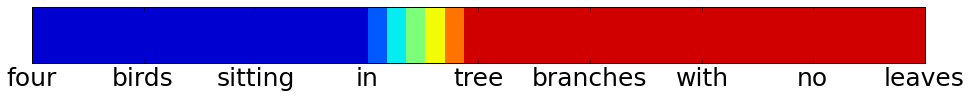
\includegraphics[scale=0.25]{dimensions/tree} \\
%\hline
%\multirow{1}{*}{\begin{sideways}\sf wii\end{sideways}} & 
% 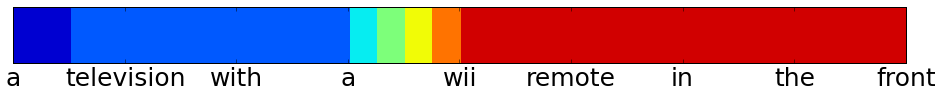
\includegraphics[scale=0.25]{dimensions/wii}  \\
%\hline
%\multirow{2}{*}{\begin{sideways}\sf next\end{sideways}} & 
%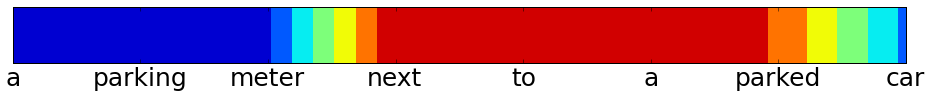
\includegraphics[scale=0.25]{dimensions/nextoacarvis} \\
%& 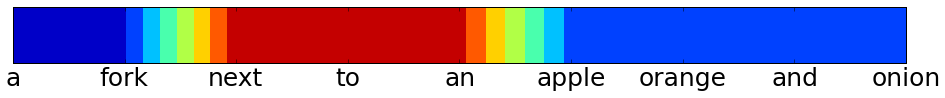
\includegraphics[scale=0.25]{dimensions/nexttoanvis}  \\
%\hline
%\hline
%\multirow{3}{*}{\begin{sideways}\sf Number\end{sideways}} & 
%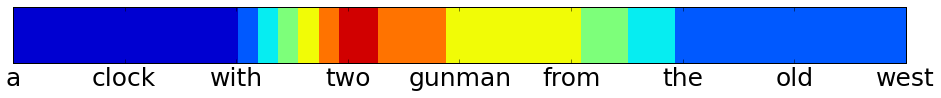
\includegraphics[scale=0.25]{dimensions/twogunmanvis}  \\
%& 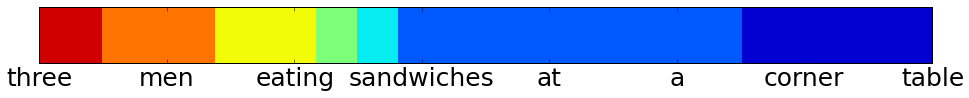
\includegraphics[scale=0.25]{dimensions/threemeneatingvis} \\
%& 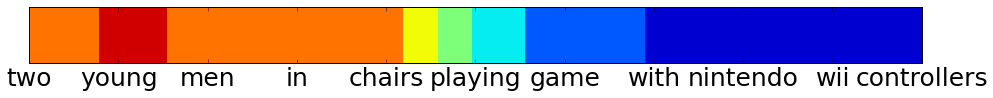
\includegraphics[scale=0.25]{dimensions/twoyoungmenvis} \\
%\hline
%\multirow{5}{*}{\begin{sideways}\sf and\end{sideways}} & 
%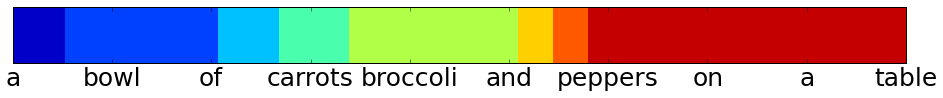
\includegraphics[scale=0.25]{dimensions/broccoliandpeppers}    \\
%& 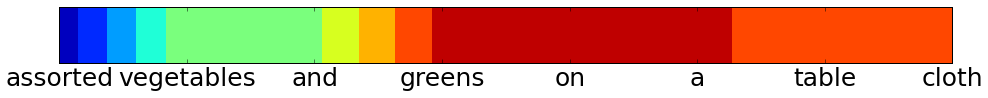
\includegraphics[scale=0.25]{dimensions/andgreensvis}  \\
%& 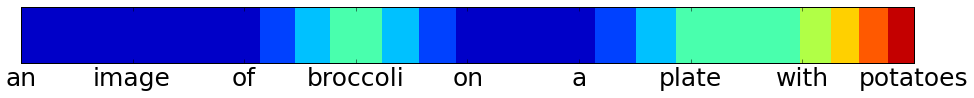
\includegraphics[scale=0.25]{dimensions/broccolipotatoes}      \\
%
%
%\end{tabular}
%
%\caption{Hidden units of {\sc Visual} active for meaningful constructions.
%The red end of the spectrum corresponds to higher activation values of the hidden unit.}
%\label{fig:dimheat}
%\end{figure}
%
\subsection{Lexical versus abstract contexts}
\label{sec:contexts}

We would like to further analyze the kinds of linguistic features that the
hidden dimensions of RNNs encode. Previous work  
\cite{karpathy2015visualizing,li2015convergent} has shown that in response 
to the task the networks are trained for, individual dimensions in the hidden layers of 
RNNs can become {\it specialised} in responding to certain types of triggers, including 
the tokens or token types at each time step, as well as the preceding context of
each token in the input sentence.
%that individual hidden dimensions of RNNs encode. 
%As discussed in the previous section, some of the analyzed units are sensitive to 
%lexical features, whereas others seem to respond to structural properties of the 
%input contexts. 

Here we perform a further comparison between the models based on the hypothesis 
that due to their different objectives, the activations of the dimensions of the last 
hidden layer of {\sc Visual} are more characterized by semantic relations within 
contexts, whereas the hidden dimensions in {\sc Textual} and {\sc LM} are 
more focused on extracting syntactic patterns. In order to quantitatively test this 
hypothesis, we measure the strength of association between activations of hidden 
dimensions and either lexical (token n-grams) or structural (dependency label n-grams) types 
of context. 

For each pathway, we define $A_i$ as a discrete random variable corresponding 
to a binned activation over time steps at hidden dimension $i$, and $C$ 
as a discrete random variable indicating the context 
(where $C$ can be of type `word trigram' or `dependency label bigram', for example). 
The strength of association between $A_i$ and $C$ can be measured 
by their mutual information:
\[
\mathrm{I}(A_i;C) = \sum_{a\in{A_i}}\sum_{c\in{C}} p(a,c)\log\left(\frac{p(a,c)}{p(a)p(c)}\right) 
\]
Similarly to \namecite{li2015convergent}, the activation value
distributions are discretized into percentile bins per dimension, such
that each bin contains 5\% of the marginal density. For context types,
we used unigrams, bigrams and trigrams of both dependency labels and
words. Figure~\ref{fig:raw_mutual} shows the distributions of the
mutual information scores for the three networks and the six context
types. Note that the scores are not easily comparable between context
types, due the different support of the distributions; they are,
however, comparable across the networks. The figure shows {\sc LM} and
{\sc Textual} as being very similar, while {\sc Visual} exhibits a
different distribution. We next compare the models' scores pairwise to
pinpoint the nature of the differences.
\begin{figure}
  \centering
  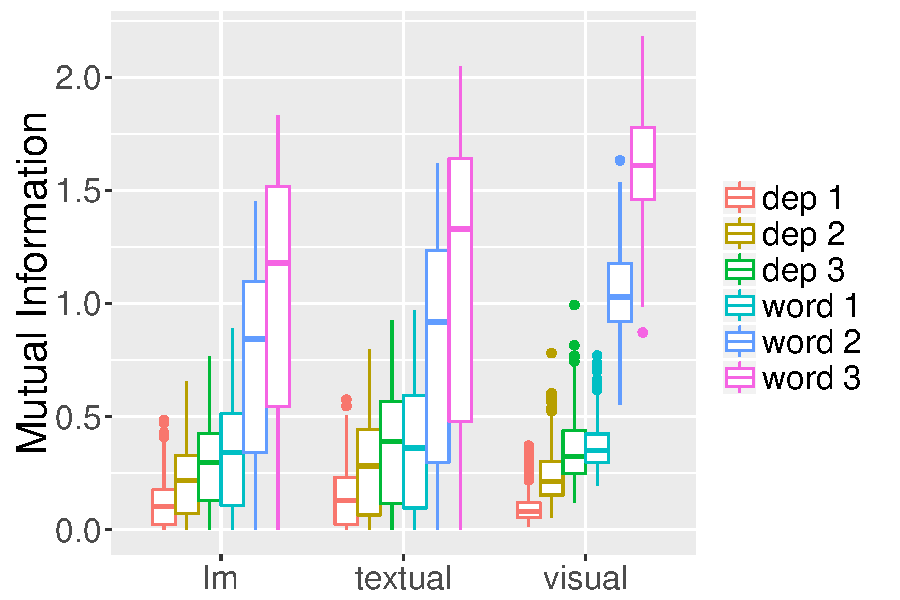
\includegraphics[scale=0.6]{raw_mutual.pdf}
  \caption{Distributions of the mutual information scores for the three networks and the six context types.}
  \label{fig:raw_mutual}
\end{figure}

We use the notation $\mathrm{MI}^\mathit{LM}_C$,  $\mathrm{MI}^T_C$ and  $\mathrm{MI}^V_C$ 
to denote the median mutual information score over all dimensions of {\sc LM}, {\sc Textual} and {\sc Visual} 
respectively, when considering context $C$. 
% We first calculate $\mathrm{MI}^{T}_{C}$ and $\mathrm{MI}^{V}_{C}$ 
% for all six context types, and observe that the median mutual information between
% activation values of the hidden units of {\sc Textual} is higher than for {\sc Visual}.
% To statistically test the observation, we used the Wilcoxon rank-sum test and performed 
% 6 pairwise comparisons between the two models. After applying Bonferroni 
% correction we found that there is a significant difference between the models in all 
% conditions ($p< 0.008$). This suggests that in general, there is a stronger 
% relationship between the activation values of the hidden units of {\sc Textual} and the 
% n-grams they co-occur with.
We then compute log ratios $\log(\mathrm{MI}^{T}_{C}/\mathrm{MI}^{V}_{C})$ and $\log(\mathrm{MI}^\mathit{LM}_{C}/\mathrm{MI}^{T}_{C})$
for all six context types $C$. In order to quantify variability we bootstrap this statistic with
5000 replicates. Figure~\ref{fig:mi-boot} shows the resulting bootstrap distributions 
for uni-, bi-, and trigram contexts, in the word and dependency conditions. 


The clear pattern is that for {\sc Textual} versus {\sc Visual}, the
log ratios are much higher in the case of the dependency contexts,
with no overlap between the bootstrap distributions. Thus, in general,
the size of the relative difference between {\sc Textual} and {\sc
  Visual} median mutual information score is much more pronounced for
dependency context types.  This suggests that features that are
encoded by the hidden dimensions of the models are indeed different, and
that the features encoded by {\sc Textual} are more associated with
syntactic constructions than in the case of {\sc Visual}. In contrast,
when comparing {\sc LM} with {\sc Textual}, the difference between
context types is much less pronounced, with distributions
overlapping. Though the difference is small, it goes in the direction
of the dimensions of the {\sc Textual} model showing higher
sensitivity towards dependency contexts.

\begin{figure}
  \centering
  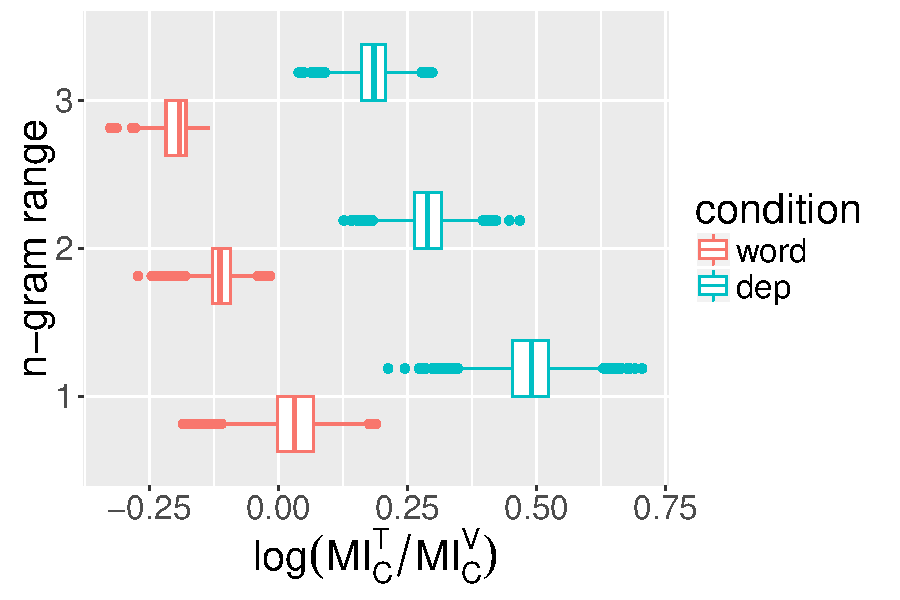
\includegraphics[scale=0.4]{bootstrappedMI.pdf}
  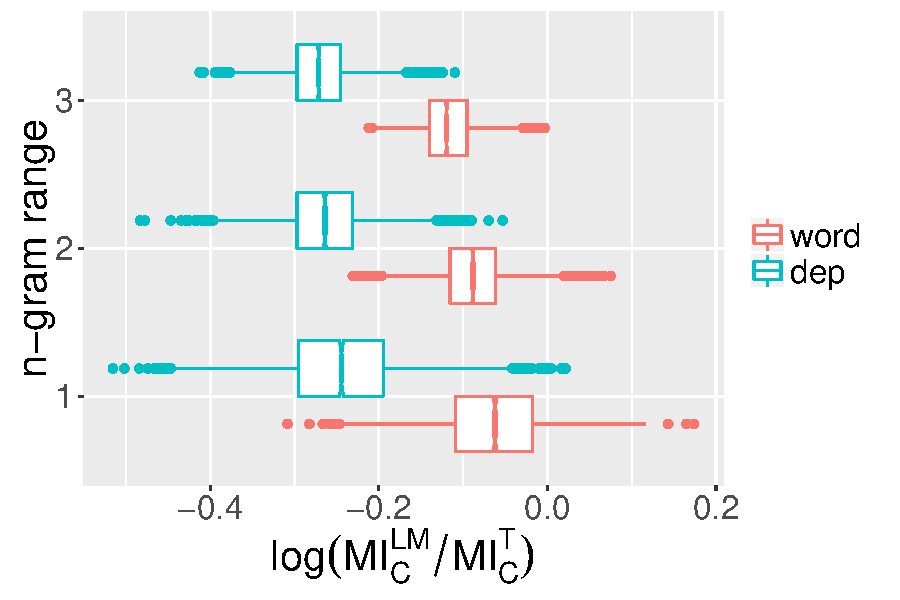
\includegraphics[scale=0.4]{bootstrappedMI2.pdf}
  \caption{Bootstrap distributions of log ratios of median mutual
    information scores for word and dependency contexts. Left: {\sc Textual}
      vs {\sc Visual}; right: {\sc LM} vs {\sc Textual}}
  \label{fig:mi-boot}
  \vspace{-.2cm}
\end{figure}


%\todo[inline]{Add and discuss sample contexts for each model here.}

The mutual information scores can be used to pinpoint specific
dimensions of the hidden activation vectors which are strongly
associated with a particular type of
context. Table~\ref{tab:mi-examples} lists for each network the
dimension with the highest mutual information score with respect to
the {\it dependency trigram} context type, together with the top
five contexts where these dimensions carry the highest value. In spite
of the quantitative difference between the networks discussed above,
the dimensions which come up top seem to be capturing something quite
similar for the three networks: (a part of) a construction with an
animate root or subject modified by a participle or a prepositional
phrase, though this is somewhat less clean-cut for the {\sc Visual}
pathway where only two out of five top context clearly conform to this
pattern.  Other interesting templates can be found by visual
inspection of the contexts where high-scoring dimensions are active;
for example, dimension 324 of {\sc LM} is high for {\it word bigram} 
contexts including
{\it people preparing, gets ready, man preparing, woman preparing,
  teenager preparing}.

\begin{table}
  \centering
  \caption{Dimensions most strongly associated with the dependency trigram context type, and the top five contexts in which these dimensions have high values.} 
\label{tab:mi-examples}
\begin{tabular}{lll}
  Network            & Dimension & Examples         \\\hline
  {\sc LM}           & 511       & cookie/pobj attached/acl to/prep \\
                     &           & people/pobj sitting/acl in/prep \\
                     &           & purses/pobj sitting/pcomp on/prep\\
                     &           & and/cc talks/conj on/prep \\
                     &           & desserts/pobj sitting/acl next/advmod \\\hline
  {\sc Textual}      & 735       & male/root on/prep a/det        \\
                     &           & person/nsubj rides/root a/det   \\
                     &           & man/root carrying/acl a/det \\
                     &           & man/root on/prep a/det         \\
                     &           & person/root on/prep a/det       \\\hline
% {\sc Textual}      & dep 3 & 1008      & bears/pobj posing/acl near/prep \\
%                    &       &           & of/prep people/pobj in/prep      \\
%                    &       &           & his/poss head/dobj on/prep       \\
%                    &       &           & food/compound dish/root with/prep    \\
%                    &       &           & living/compound room/root with/prep  \\\hline
  {\sc Visual}       &  875      & man/root riding/acl a/det \\
                     &           & man/root wearing/acl a/det \\
                     &           & is/aux wearing/conj a/det \\
                     &           & a/det post/pobj next/advmod \\
                     &           & one/nummod person/nsubj is/aux \\

% {\sc LM}           & word 3 & 38        & a professional baseball \\
%                    &        &           & rustic looking living \\
%                    &        &           & a white teddy         \\
%                    &        &           & a clean living        \\
%                    &        &           & a white beige         \\\hline
%                    % & word 3 & 117       & soccer on top \\
%                    % &        &           & ball on top \\
%                    % &        &           & frisbee on top \\
%                    % &        &           & racket playing on \\
%                    % &        &           & grazing on lush \\
% {\sc Textual}      & word 3 &  764      & down a rocky \\
%                    &        &           & on a busy \\
%                    &        &           & very busy street \\
%                    &        &           & on a busy \\
%                    &        &           & is playing tennis \\\hline
% {\sc Visual}       & word 3 & 215       & electric tooth brush \\
%                    &        &           & and a girl \\
%                    &        &           & man leans down \\
%                    &        &           & little kitty laying \\
%                    &        &           & her left hand \\

\end{tabular}
\end{table}
%Figure~\ref{fig:entropybox} shows two sets of box plots representing the mutual 
%information distributions for token and deprel n-gram contexts ($n\in{1,2,3}$). 
%Results show that in fact the medians for {\sc Textual} are higher than for {\sc Visual}, 
%especially when $C$ represents deprel n-grams. This means that {\sc Textual}
%dimensions are in fact more specialized towards reacting to syntactic contexts. 




%Motivated by the intuitively interpretable context-lists describing the function of 
%hidden dimensions using the magnitude of activations values, we turn to gain more 
%insight into the difference between TEXTUAL and VISUAL. The results in Section 
%LOGISTIC suggest that the hidden representations of TEXTUAL contain more 
%information about the syntactic structure of the input sentences than VISUAL. 
%Based on this insight we conjecture that while the activity of hidden dimensions of 
%VISUAL are characterized by semantic relationships between contexts the 
%neurons of TEXTUAL are more focused on extracting syntactic patterns. To 
%validate this assumption we consider the frequency distributions of the top 10,000 
%highest activating token and dependency relation uni-, bi- and tri-gram contexts for 
%both models. Here we make two simplifying assumptions: a) as before the 
%magnitude of the activations value suggests "importance", b) we do not take into 
%consideration the rank of the contexts. We compute the entropy of these frequency 
%distributions to measure how specialized each dimensions is to specific contexts. 
%Figure \ref{fig:entropybox} compares the distribution of entropy scores of the 
%individual hidden dimensions between TEXTUAL and VISUAL. The boxplots 
%comparing the models on dependency relations - bottom row - and tokens - top row 
%- shows that in all conditions - uni-, bi-, tri-gram - the median entropy scores for the 
%hidden dimensions VISUAL are higher than for TEXTUAL. This result suggests 
%that the features extracted from the sentences by TEXTUAL resemble syntactic 
%constructions more than in case of VISUAL. To statistically test the hypothesis we 
%use the Wilcoxon rank-sum test with and perform 6 pairwise comparisons between 
%the two models on both dependency relation and token contexts. After applying 
%Bonferroni correction we find that there is a significant difference between the 
%models in all conditions except for token bi-grams - $p< 0.05/6 = 0.008$.	

%\begin{figure*}[t]

%\begin{tabular}{ccc}
%\includegraphics[scale=0.2]{unique/MItoken1} & \includegraphics[scale=0.2]
%{unique/MItoken2} & \includegraphics[scale=0.2]{unique/MItoken3} \\
%\includegraphics[scale=0.2]{unique/MIdeprel1} & \includegraphics[scale=0.2]
%{unique/MIdeprel2} & \includegraphics[scale=0.2]{unique/MIdeprel3}
%\end{tabular}

%\caption{The distribution of the Mutual Information scores for each hidden dimension of 
%{\sc Visual} and {\sc Textual}. Plots on the top row show scores for token n-grams, and on 
%the bottom row for dependency relation n-grams.}
%\label{fig:entropybox}
%\end{figure*}




%\input{visualization}